\documentclass[a4paper,12pt]{book}

% Paquetes de Latex
\usepackage[left=2.25cm,right=2.25cm,top=2.5cm,bottom=2.5cm]{geometry}
%\usepackage[sc]{mathpazo}
\linespread{1.05}
\usepackage[T1]{fontenc}
\usepackage[utf8]{inputenc}
\usepackage[spanish, es-tabla, english]{babel}
\decimalpoint
\usepackage{graphicx}
\usepackage{xcolor}
\usepackage{colortbl}
% Scalable fonts (para lettrine)
\usepackage{type1ec} 
\usepackage{lettrine}
% Cabeceras y pies de página
\usepackage{fancyhdr}
% Vertabim
\usepackage{moreverb}
% Código 
\usepackage{listingsutf8}
% Identacion y separacion de parrafos
\usepackage{parskip}
% Posicion de figuras
\usepackage{float}
% Diagramas
\usepackage[all,pdf]{xy}
% Firma digital
%\usepackage{eforms}
% Subfiguras
\usepackage{subfig}
% Hyperref
\usepackage{hyperref}
\hypersetup{
	colorlinks,%
	citecolor=black,%
	filecolor=black,%
	linkcolor=black,%
	urlcolor=black,%
	pageanchor=false
}
% URL en bibliografía
\usepackage{xurl}
% Apéndices
\usepackage{appendix}
% Múltiples columnas
\usepackage{multicol}
% Captions en multicols
\usepackage{caption}
% Títulos de capítulos
\usepackage{titlesec}
\titleformat{\chapter}[display]
{\bfseries\Large} 
{\filleft\MakeUppercase{\chaptertitlename} \Huge\thechapter} {4ex}
{\titlerule
\vspace{2ex}%
\filright} [\vspace{2ex}%
\titlerule]
% Tablas
\usepackage{tabularx}
\usepackage{booktabs}
% Tablas largas
\usepackage{longtable}
% Columnas de más de una fila en las tablas
\usepackage{multirow}
% Fechas
\usepackage{datetime}

\usepackage[acronym, toc]{glossaries}
\usepackage{amsmath}
\usepackage{amssymb,amsfonts,latexsym,cancel}

% Unidades
\usepackage{siunitx}
% Figuras
\usepackage{standalone}
\usepackage{tikz}
\usetikzlibrary{
    automata, 
    positioning, 
    arrows, 
    shapes.geometric,  
    shapes.symbols, 
    external
}

% Configuración de la bibliografía
\usepackage[
    bibstyle=ieee,
    citestyle=numeric,
    isbn=true,
    doi=false,
    sorting=none,
    url=true,
    bibencoding=utf8,
    backend=bibtex
]{biblatex}
\addbibresource{bibliografia.bib}
\usepackage{xpatch}
\xpatchbibdriver{online}
  {\printtext[parens]{\usebibmacro{date}}}
  {\iffieldundef{year}
    {}
    {\printtext[parens]{\usebibmacro{date}}}}
  {}
  {\typeout{There was an error patching biblatex-ieee (specifically, ieee.bbx's @online driver)}}
  
\setcounter{biburllcpenalty}{100}
\setcounter{biburlucpenalty}{200}
\setcounter{biburlnumpenalty}{100}
  
% Configuración de TikZ 
\makeatletter
\tikzset{
    database top segment style/.style={draw},
    database middle segment style/.style={draw},
    database bottom segment style/.style={draw},
    database/.style={
        path picture={
            \path [database bottom segment style]
                (-\db@r,-0.5*\db@sh) 
                -- ++(0,-1*\db@sh) 
                arc [start angle=180, end angle=360,
                    x radius=\db@r, y radius=\db@ar*\db@r]
                -- ++(0,1*\db@sh)
                arc [start angle=360, end angle=180,
                    x radius=\db@r, y radius=\db@ar*\db@r];
            \path [database middle segment style]
                (-\db@r,0.5*\db@sh) 
                -- ++(0,-1*\db@sh) 
                arc [start angle=180, end angle=360,
                    x radius=\db@r, y radius=\db@ar*\db@r]
                -- ++(0,1*\db@sh)
                arc [start angle=360, end angle=180,
                    x radius=\db@r, y radius=\db@ar*\db@r];
            \path [database top segment style]
                (-\db@r,1.5*\db@sh) 
                -- ++(0,-1*\db@sh) 
                arc [start angle=180, end angle=360,
                    x radius=\db@r, y radius=\db@ar*\db@r]
                -- ++(0,1*\db@sh)
                arc [start angle=360, end angle=180,
                    x radius=\db@r, y radius=\db@ar*\db@r];
            \path [database top segment style]
                (0, 1.5*\db@sh) circle [x radius=\db@r, y radius=\db@ar*\db@r];
        },
        minimum width=2*\db@r + \pgflinewidth,
        minimum height=3*\db@sh + 2*\db@ar*\db@r + \pgflinewidth,
    },
    database segment height/.store in=\db@sh,
    database radius/.store in=\db@r,
    database aspect ratio/.store in=\db@ar,
    database segment height=0.1cm,
    database radius=0.25cm,
    database aspect ratio=0.35,
    database top segment/.style={
        database top segment style/.append style={#1}},
    database middle segment/.style={
        database middle segment style/.append style={#1}},
    database bottom segment/.style={
        database bottom segment style/.append style={#1}}
}
\makeatother

\tikzset{
    ->,  % makes the edges directed
    >=stealth', % makes the arrow heads bold
    every state/.style={thick, fill=gray!10}, % sets the properties for each ’state’ node
    initial text=$ $, % sets the text that appears on the start arrow
}


% Definimos unidades
\DeclareSIUnit{\byte}{B}

\includeonly{
    %resumen,
    %abstract,
    Introduccion,
    %Estado_del_Arte,
    %Objetivos_Metodologia,
    %Diseno_Resolucion,
    %Resultados,
    %Conclusiones
}

\newcommand{\HRule}{\rule{\linewidth}{0.5mm}}
\renewcommand{\chaptermark}[1]{\lhead[{\sc{\chaptername\ #1}}]{}}
\renewcommand{\sectionmark}[1]{\rhead[ ]{{\thesection.\ #1}}}

% Nuevo tipo de columnas
\renewcommand\tabularxcolumn[1]{m{#1}}% for vertical centering text in X column
\newcolumntype{Y}{>{\centering\arraybackslash}X}

% Definición colores
\definecolor{verdedato}{RGB}{78,173,50}
\definecolor{rojodato}{RGB}{234,51,35}
\definecolor{azuldato}{RGB}{0,0,200}

\definecolor{codegreen}{RGB}{184,215,163}
\definecolor{codegray}{rgb}{0.5,0.5,0.5}
\definecolor{codepurple}{rgb}{0.58,0,0.82}
\definecolor{backcolour}{rgb}{0.95,0.95,0.92}

\definecolor{azuldiagrama}{RGB}{93,160,242}
\definecolor{verdediagrama}{RGB}{124,244,111}
\definecolor{rojodiagrama}{RGB}{204,73,53}
\definecolor{naranjadiagrama}{RGB}{209,139,69}
\definecolor{blancodiagrama}{RGB}{237,247,211}

\definecolor{azulclasificador}{RGB}{181,199,230}
\definecolor{verdeclasificador}{RGB}{197,224,181}
\definecolor{rojoclasificador}{RGB}{248,204,175}

% Code Listing Configuration
\lstdefinestyle{mystyle}{
    backgroundcolor=\color{white},   
    commentstyle=\color{gray},
    keywordstyle=\color{blue},
    numberstyle=\tiny\color{codegray},
    stringstyle=\color{gray},
    basicstyle=\ttfamily\scriptsize,
    breakatwhitespace=false,         
    breaklines=true,                 
    captionpos=b,                    
    keepspaces=true,                 
    numbers=left,                    
    numbersep=5pt,                  
    showspaces=false,                
    showstringspaces=false,
    showtabs=false,                  
    tabsize=3
} 
\lstset{language=Python, style=mystyle, inputencoding=utf8/latin1, mathescape}
\lstset{%
        inputencoding=utf8,
        extendedchars=true,
        literate=%
        {é}{{\'{e}}}1
        {è}{{\`{e}}}1
        {ê}{{\^{e}}}1
        {ë}{{\¨{e}}}1
        {É}{{\'{E}}}1
        {Ê}{{\^{E}}}1
        {û}{{\^{u}}}1
        {ù}{{\`{u}}}1
        {â}{{\^{a}}}1
        {à}{{\`{a}}}1
        {á}{{\'{a}}}1
        {ã}{{\~{a}}}1
        {Á}{{\'{A}}}1
        {Â}{{\^{A}}}1
        {Ã}{{\~{A}}}1
        {ç}{{\c{c}}}1
        {Ç}{{\c{C}}}1
        {õ}{{\~{o}}}1
        {ó}{{\'{o}}}1
        {ô}{{\^{o}}}1
        {Õ}{{\~{O}}}1
        {Ó}{{\'{O}}}1
        {Ô}{{\^{O}}}1
        {î}{{\^{i}}}1
        {Î}{{\^{I}}}1
        {í}{{\'{i}}}1
        {Í}{{\'{I}}}1
        {ñ}{{\~n}}1
        {ú}{{\'{u}}}1
}

\begin{document}
\selectlanguage{spanish}
\title{Identificación de dispositivos IoT a través de huellas hardware}
\author{Sergio Marín Sánchez}
\newdate{fecha}{4}{7}{2022}

\begin{titlepage}
 
\begin{center}
 
% Upper part of the page
\vfill


\includegraphics[height=0.5\textwidth]{escudo}\\[2.5cm]
 
\textsc{\LARGE Universidad de Murcia}\\[0.5cm]
 
\textsc{\Large Trabajo Final de Grado}\\[0.5cm]
 
% Title
\HRule \\[0.4cm]
{ \huge \bfseries Identificación de dispositivos IoT}\\[0.4cm]
{ \huge \bfseries  a través de huellas hardware}\\[0.4cm]
\HRule \\[1.5cm]
 
% Author and supervisor
\begin{minipage}{0.4\textwidth}
\begin{flushleft} \large
\emph{Autor:}\\
Sergio \textsc{Marín Sánchez}\\
\href{mailto:sergio.marins@um.es}{sergio.marins@um.es}
\end{flushleft}
\end{minipage}
\begin{minipage}{0.4\textwidth}
\begin{flushright} \large
\emph{Tutores:} \\
Gregorio \textsc{Martínez Pérez}\\
\href{mailto:gregorio@um.es}{gregorio@um.es}\\
Pedro Miguel \textsc{Sánchez Sánchez}\\
\href{mailto:pedromiguel.sanchez@um.es}{pedromiguel.sanchez@um.es}
\end{flushright}
\end{minipage}
 
\vfill
 
% Bottom of the page
{\large \displaydate{fecha}}
 
\end{center}
 
\end{titlepage}

\let\cleardoublepage\newpage

\clearpage{\pagestyle{empty}\cleardoublepage}

% Agradecimientos
%!TEX root = proyecto.tex

\pagestyle{empty}
\newgeometry{left=12.25cm, textwidth=6cm}
\phantom{a}
\vfill
\begin{flushright}
\textit{%
%
Me gustaría expresar mi agradecimiento a todos los amigos, profesores y familia que han hecho posible que llegue a este punto.
%
}
\end{flushright}
\vfill
\restoregeometry

\clearpage{\pagestyle{empty}\cleardoublepage}

\pagestyle{plain}
\setcounter{page}1
\setcounter{secnumdepth}{4}	%Profundidad de la numeracion del indice
\setcounter{tocdepth}{2}	%Profundidad del indice

\tableofcontents
\clearpage{\pagestyle{empty}\cleardoublepage}

\listoffigures
\clearpage{\pagestyle{empty}\cleardoublepage}

\listoftables
\clearpage{\pagestyle{empty}\cleardoublepage}

\setlength{\parindent}{18pt}

% Declaracion de originalidad
%%!TEX root = TFG.tex

\pagestyle{plain}

\chapter*{Declaración firmada sobre la originalidad del trabajo}
\addcontentsline{toc}{chapter}{Declaración firmada sobre la originalidad del trabajo}

D. Sergio Marín Sánchez, con DNI 49197868V, estudiante de la titulación de Grado en Ingeniería Informática de la Universidad de Murcia y autor del TF titulado ``Identificación de dispositivos IoT a través de huellas hardware''.

De acuerdo con el Reglamento por el que se regulan los Trabajos Fin de Grado y de Fin de Máster en la Universidad de Murcia (aprobado C. de Gob. 30-04-2015, modificado 22-04-2016 y 28-09-2018), así como la normativa interna para la oferta, asignación, elaboración y defensa delos Trabajos Fin de Grado y Fin de Máster de las titulaciones impartidas en la Facultad de Informática de la Universidad de Murcia (aprobada en Junta de Facultad 27-11-2015).

\noindent DECLARO:

Que el Trabajo Fin de Grado presentado para su evaluación es original y de elaboración personal. Todas las fuentes utilizadas han sido debidamente citadas. Así mismo, declara que no incumple ningún contrato de confidencialidad, ni viola ningún derecho de propiedad intelectual e industrial. \\

\begin{center}
\begin{tabular}{c}
    Murcia, a \displaydate{fecha} \\
    \sigField{Firma}{5cm}{3cm} \\
    Fdo.: Sergio Marín Sánchez \\
    \textit{Autor del TF}
\end{tabular}
\end{center}

\clearpage{\pagestyle{empty}\cleardoublepage}

% Resumen en castellano
%!TEX root = TFG.tex

\chapter*{Resumen}
\addcontentsline{toc}{chapter}{Resumen} \label{chap:resumen}

En este proyecto se ha diseñado una solución capaz de identificar dispositivos conectados en red local en base a las diferencias entre sus relojes internos comparados con un reloj que se fija como referencia. Con esto, ha sido creado un mecanismo que permitirá gestionar de una mejor manera los dispositivos autorizados a realizar ciertas funciones o estar conectados con otros dispositivos de la red.

Este trabajo se puede dividir en cuatro partes. En primer lugar se realiza una fase de diseño de la arquitectura de la solución que se propone. En esta propuesta de solución se identifican las etapas requeridas para llevar a cabo el desarrollo de este proyecto. En la siguiente parte se explica la obtención de los datos, para lo que han sido utilizados 5 dispositivos iguales en hardware y software (Raspberry Pi 4 Model B). De estos dispositivos se obtienen marcas de tiempo cada segundo de dos formas distintas. Por otro lado, se tiene la fase de análisis estadístico de los datos obtenidos, en el que se generan nuevos datos a partir de los previos. Por último, está la fase del desarrollo de un modelo de Machine Learning que sea capaz de automatizar todo el proceso de distinguir los dispositivos partiendo de los datos estadísticos que se han obtenido previamente.

Para obtener los datos se ha hecho uso de una arquitectura cliente-servidor entre los dispositivos a analizar y el dispositivo observador, con el fin de controlar el ritmo de envío de los paquetes. Las capturas se han realizado de dos formas, en secuencial y en paralelo. Secuencialmente hace referencia a que primero se obtienen todas las marcas de tiempo de un dispositivo y posteriormente se analiza el siguiente. Por otro lado, paralelamente hace referencia a que se obtienen marcas de tiempo de todos los dispositivos simultáneamente.

Una vez se tienen todas las marcas de tiempo, se obtienen sus desviaciones respecto al dispositivo que se designó como referencia. De estas desviaciones se obtiene su incremento entre cada dos puntos. Comparando las muestras individual y paralela entre sí mediante gráficos de cajas, se aprecia que los datos de la muestra individual presentan una estructura que no se asemeja tanto a los datos esperados de estos experimentos. Lo esperado sería encontrar la desviación con valores centrados en 0 (lo que se da en ambas muestras) y muy similares entre todos los dispositivos. Es en este último requisito que la muestra individual no se comporta de la forma esperada y, por tanto, a partir de este punto sólo se usarán los datos de la muestra paralela. Estos valores son agrupados mediante una ventana deslizante de 1 minuto, que equivale a 60 paquetes (se toman muestras cada segundo), y de cada uno de estos grupos se obtienen diversas variables estadísticas.

Antes de proceder con la sección dedicada a Machine Learning, se deben eliminar las variables estadísticas que presenten correlación, de esta forma se reduce la cantidad de variables que se usarán para los entrenamientos.

Una vez se tienen las variables estadísticas finales, se analizarán los algoritmos de Machine Learning que han sido escogidos para este trabajo. Los algoritmos que se van a analizar son por una parte de clasificación, como Random Forest, \acrfull{mlp}, \acrfull{knn}, Naive Bayes, Árboles de decisión y \acrfull{svm} con kernel lineal; y por otra, de detección de anomalías no supervisados como, Isolation Forest, \acrfull{lof} y \acrfull{ocsvm}.

Para comparar los modelos de clasificación entre sí se usará el modelo entrenamiento/validación/test como forma de dividir los datos. Se entrenarán todos los modelos con el conjunto de entrenamiento y se comprobará su capacidad de generalización con el conjunto de validación. A la hora de entrenar los modelos se comprobarán diferentes parrillas de hiperparámetros para ajustar los modelos lo más posible a los datos de entrenamiento.

A la hora de particionar el conjunto de datos de cara a los entrenamientos de los algoritmos se ha seguido un método propio, con el fin de no perder la correlación temporal que presenta la muestra. Para dividir el conjunto se selecciona una muestra aleatoria de los datos del tamaño deseado, y posteriormente se restablece el orden original de los mismos. De esta forma se consigue reducir el tamaño del conjunto de datos y conservar la correlación temporal de mismos.

Por otra parte, los algoritmos de detección de anomalías han sido entrenados por cada dispositivo, en lugar de todos a la vez. Se ha usado una parte de los datos de cada dispositivo para entrenar el algoritmo, y posteriormente se ha evaluado su rendimiento el resto de los datos de ese dispositivo y con el resto de dispositivos, esto último de forma separada.

Al realizar estos entrenamientos se puede apreciar que los modelos basados en árboles son los mejores, tanto árboles de decisión (95.92\%) como Random Forest (99.22\%). Finalmente se elige el algoritmo de Random Forest y se procede a entrenarlo con la totalidad de los datos de entrenamiento y los hiperparámetros usados anteriormente. 

Al realizar estos entrenamientos se ha apreciado que los algoritmos de detección de anomalías no obtienen resultados elevados. Por contra, algunos de los algoritmos de clasificación sí que son capaces de obtenerlos, en concreto, los basados en árboles (Árboles de decisión y Random Forest). Este último es el algoritmo elegido para generar un modelo de identificación final.

Como resultado se tiene que este último modelo de Random Forest final obtiene un valor final de Accuracy de 99.38\%, de Recall de 99.39\% y de $f$-score de 99.38\%. Gracias a este resultado, se ha llegado a la conclusión de que es posible automatizar el proceso de distinguir dispositivos idénticos de forma remota.

Con vistas a futuro, se puede concluir que este trabajo aporta una solución que potencialmente puede ayudar a la lucha contra la ciberdelicuencia, pero se deben resolver algunos inconvenientes. Por un lado, hay servicios que modifican constantemente el reloj del sistema y esto dificulta la tarea de crear una huella para los dispositivos. Por otro lado, y tal vez el más importante, es que esta huella ha de ser creada para cada dispositivo concreto, lo cual es una labor incomensurable.



\clearpage{\pagestyle{empty}\cleardoublepage}

% Resumen en inglés
%!TEX root = TFG.tex

\chapter*{Extended abstract}
\addcontentsline{toc}{chapter}{Extended abstract} \label{chap:abstract}

Nowadays, the number of devices connected to the internet has increased significantly due to smartphones, IoT devices, autonomous cars, etc. These devices must be always connected to the internet to be able to perform the actions for which they are intended. 

These kinds of devices contain and share a lot of information about the people who use them. For this reason, many people try to get this data for purposes that may not be legal. One way to do it would be to pretend that you are the device of the person that you want to access. In order to succeed, it is necessary to change all the identifiers to those that the criminal wants to impersonate. By doing this, people will connect to the criminal's device without being aware of it.


Devices that have the same hardware and software components are not exactly the same, there are some details during the manufacturing process that cannot be copied. Taking advantage of this, a system with the ability to identify those differences was created and as a consequence, between many devices too.

In this work, \acrfull{iot} devices were used to perform the objectives. These are devices capable of connecting to the Internet, collecting data and exchanging this data on their own. The concept of IoT devices was proposed by Kevin Ashton in 1999.

These types of devices need a different network architecture than normal devices because of their requirements regarding security and \acrfull{qos}. Different proposals have been given from multiple research. One of them is the one from Ibrar Yaqoob et al. \cite{yaqoob2017internet} where they propose a three-layer architecture: application, transport, and sensing.

As mentioned, in this work a system that can identify those details mentioned above was created. Many studies have already researched device identification, but a lot of times they focus on distinguishing devices, but these investigations do not bring the focus to these devices that are identical in both hardware and software.

Most of the read approaches use Machine Learning, specifically supervised learning algorithms, to identify between different devices, and they use this capacity to identify devices for security purposes, for example, giving access to a private network or knowing if an access point may be malicious. The results of the read approaches are situated between 42\% and nearly 100\% of accuracy value. 

In this research, to identify different devices, several timestamps were taken from every device under analysis and, after that, their differences from one to the next one were calculated. These timestamps contain the amount of time since the device was turned on. The small differences that distinguish these devices make that as time goes by, their internal clocks fluctuated. This error accumulated over time and became more noticeable.

To achieve this work's objectives an architecture for how this work is developed was proposed. This architecture can be divided into two parts. On the one hand, there are devices that generate all the data and share it. On the other hand, there is an external device whose purpose is to collect the data received from the other devices, analyse and process it as well as adjust the Machine Learning algorithms that have been used. This external device also evaluates the Machine Learning models that have been trained yet and additionally it compares them too. This architecture performs all the following stages:

\begin{enumerate}[label=\Alph*)]
    \item \textbf{Set up stability conditions}. This stage performs one fundamental thing which is preparing all devices that are going to be tested. The devices' internal clocks have been set to a fixed frequency. In addition, the \acrshort{ntp} service has to be disabled. 
    \item \textbf{Data gathering}. In this stage, every second, each device under analysis generates a timestamp from its internal clock and sends it to the external device. This stage repeats for the established time, which is a period long enough. 
    \item \textbf{Data analysis and processing}. In this stage, the external device receives all the timestamps from the devices under analysis and it calculates the increase between every two consecutive timestamps. With all these timestamps' increasing values a dataset is built by the external device. Using this dataset, and a sliding window, various statistical values are obtained which are representative of the window in question. Some of these statistical value may be correlated, that's why those which are correlated are going to be removed from the dataset, except one of them which act as a representative value.
    \item \textbf{Model generation}. In this stage the different Machine Learning algorithms are selected. In this work supervised learning algorithms for classification are used as well as unsupervised learning anomaly detection algorithms. Once all the algorithms are selected, it is needed to adjust their hyperparameters in order to make the resulting models fit the data of this work in the best possible way.
    \item \textbf{Model evaluation}. In this last stage, all the metrics, which are going to be used to compare the different models with each other, are selected. Classification algorithms and anomaly detection algorithms do not use the same metrics to be compared. The resulting metrics are obtained from each trained model and then all these models are compared between them.
\end{enumerate}


The test scenario made for this project consists of six \acrshort{iot} devices connected to a local network. One of them acted as a client and the others acted as servers. Every second the client sent a timestamp request to the servers, and they replied with it. When the client received this timestamp, it saved it as a record: ``(time from the start), (client's ignition time), (server's ignition time), (time difference), (server IP)''. The client's time was taken as a reference, and the differences were analysed between the other devices and the client.


The first problem appeared at this time. Taking into account that very small differences were analysed, they might have great accuracy of the times. Initially, it was thought that the best option was using the timestamps contained in the headers of the TCP and ICMP protocols. This idea was discarded since these headers have few bytes and with them, it can only represent times in milliseconds, which does not provide enough information. For this reason, it was decided to use the body section of the packets; to be able to send data of any length. In this case, it will send absolute timestamps in nanoseconds, which will be encoded with 64 bits. Finally, it was chosen the TCP protocol because, in this way, it was not necessary to start a new connection every time a timestamp was sent.


These timestamps were taken in two different ways. On the one hand, a sequential sample was taken in which it was listening for 2 hours (7200 samples) on each device, one after another. This period of time represents a 10 hours sample (36000 samples). On the other hand, a parallel sample of all devices was also carried out, and this one developed 12 hours (with 43200 samples per device). Another issue that arose at this point was that the device's internal clock was altered by other time synchronization processes, such as the NTP protocol. As a result, it was necessary to use an internal clock that changes its value in a linear way. (\texttt{steady\_clock}). This internal clock contains the number of CPU cycles since the device was switched on.

The next step was set on to the data analysis part. Firstly, the increase in the deviation between each sample of a device was obtained. In those graphs, the median was expected to be approximately 0 and the interquartile range was expected to be very similar on each device. These results were expected since identical devices are being analyzed and they do not suffer from clock skew, at least theoretically.

Looking at both graphs, the one from the sequential sample and the one from the parallel sample, the median was observed to be actually close to 0, however, the interquartile range oscillated much more in the sequential sample. Therefore, from this point on and because of the training of the models that perform the identification process, this sample was not taken into account; the focus was laid on the parallel sample.

Once it was decided which data was going to be used, the statistical values were obtained, and a 1-minute sliding window (60 samples) was used to obtain them. The statistical values that were obtained were: sum, mean, median, mode, standard deviation, interquartile range, kurtosis, skewness, maximum and minimum.

Before training the models, it was checked if there was a correlation between the different statistical values since having correlated data does not provide information. To do that, a correlation matrix between all the statistical variables was generated and those variables that have a high correlation value with another variable were eliminated. In order to train the different models, it was used the \texttt{scikit-learn} library for Python, along with utilities such as \texttt{numpy} and \texttt{pandas}. In this work it was used supervised learning algorithms, such as Decision Trees, Random Forest, \acrfull{mlp}, Naive Bayes, \acrfull{knn} and \acrfull{svm}. In addition, it was also used unsupervised learning anomaly detection algorithms, such as Isolation Forest, \acrfull{lof} and \acrfull{ocsvm}.

In order to train the different supervised algorithms and obtain the best possible results, their hyperparameters must be set. To make this adjustment, it was used a smaller set of data, but it was representative of the totality of the data since each training costs a considerable amount of time. It was used a training/validation/test model.
 
 
The set of all the data will be divided into two, one with \SI{70}{\percent} of the data and another with \SI{30}{\percent}. The training set will be used to train the final model and the test model will be used to see the generalization capacity of the model.


The process of adjusting an algorithm takes time since each algorithm has to be trained with each combination of hyperparameters that are required for being tested. For this reason, the volume of data was reduced (\SI{70}{\percent} of the total) and kept only \SI{35}{\percent} of it. This subset will also be divided into a 70/30 ratio in order to validate the results of training with data that the model had not seen before.

To make these partitions, random samples were taken, but as the data had temporal correlation, reordering them was needed so that this correlation could be kept and the models were able to recognize it. 

To adjust the hyperparameters of an algorithm, an object called grid, which allows specifying all the hyperparameters that were tested, was used. This tool is very useful since it automates the whole process of testing different hyperparameters and allows us to obtain, in a single run, the results of an algorithm with each combination of hyperparameters.

As regards anomaly detection algorithms, another scheme was used. Their hyperparameters were also adjusted similarly to the supervised ones, however, anomaly detection algorithms used only the data from one device to be trained. It was used \SI{80}{\percent} of the data from every device to train the algorithm and, after that, the algorithm was evaluated using two different tests, the remaining \SI{20}{\percent} of the device data and the \SI{20}{\percent} of all the remaining devices' data. Looking at the first test, how capable to detect the current device was shown, and with the second one, it was shown how capable of not making a mistake was the algorithm.


Once all the models had been tested, it could be seen that the ones with the best results were those that are based on trees; both Decision Trees and Random Forest.  In particular, Random Forest was the one with the best results, so, this Random Forest algorithm was chosen to be trained as the final model. 

Finally, the Random Forest algorithm with its custom hyperparameters and the training set in its completeness was the only one that have to be trained. Once this has been done, its ability to generalize is checked with the test set and it is obtained a final accuracy of \SI{99.38}{\percent}, a recall of \SI{99.39}{\percent} and an $f-score$ of \SI{99.38}{\percent}.


It can be concluded that it is possible to identify theoretically identical devices automatically, but it should be noted that all of this process has been made on a private network. If the same study had been done over the Internet, the result would have been different. This is because even if all the devices were on the same local network and only the observer was out, each timestamp of each device could be routed differently, which would cause measurement errors. A possible solution to this problem would be to take much longer samples in time, since statistically the packets between two devices will be routed most of the time along the same path, leaving those which are not, like outliers. 



\clearpage{\pagestyle{empty}\cleardoublepage}

\pagestyle{fancy}
\renewcommand{\chaptermark}[1]{\lhead[{\sc{\chaptername\ \thechapter.\ #1}}]{}}
\renewcommand{\sectionmark}[1]{\rhead[ ]{{\thesection.\ #1}}}
\renewcommand{\headrulewidth}{0.5pt}
\renewcommand{\footrulewidth}{0.5pt}

% Introduccion
%!TEX root = TFG.tex

\chapter{Introducción} \label{chap:intro}

\section{Contexto}

En los últimos años el número de dispositivos conectados a internet se ha incrementado en gran medida \cite{84Billio53:online}. Esto se debe al uso de smartphones, tablets y demás dispositivos que requieren de conexión a internet para llevar a cabo la mayoría (o la totalidad) de tareas para las que han sido diseñados.

Cada dispositivo conectado a internet tiene asociados varios identificadores, como la dirección IP y la dirección MAC. Estos identificadores deberían servir para identificar unívocamente a un dispositivo, pero en la práctica no se da esta situación. Las direcciones IP pueden cambiar automáticamente debido al direccionamiento IP dinámico (mediante servidores DHCP), pero también pueden ser modificadas por las propias personas. 

Estas modificaciones pueden ser por temas únicamente de privacidad, pero en muchas ocasiones están relacionadas con la ciberdelincuencia. Los delicuentes pueden intentar falsificar sus identificadores con el objetivo de que las personas, buscando conectarse a un servicio legítimo, acaben conectándose a sus equipos.

Los fines de esto son, por ejemplo, introducir virus en sus equipos, para realizar ataques DDoS (ataques de denegación de servicio distribuidos) mediante miles de equipos infectados, para cifrar los datos de dicho equipo (ataque de ransomware), para realizar ataques de phishing, enviando páginas visualmente idénticas a las que consulte el equipo, pero los datos sensibles de los formularios (contraseñas) pasen a disposición del atacante. Otro fin posible es el mero espionaje de los datos.

\section{Motivación}

Es en este punto en el que se requieren técnicas de comunicación seguras entre los dispositivos. Desde el punto de vista de las redes existen protocolos de comunicación segura como SSL, TLS, IPsec, etc. Pero estos dispositivos son inútiles si el equipo se quiere conectar voluntariamente al equipo atacante (esto debido al engaño que se ha comentado anteriormente).

Por estos motivos, existe la pregunta sobre cómo podemos saber a qué equipos nos estamos conectando, o qué diferencia a un dispositivo de otro en internet si ambos presentan los mismos identificadores.

Una respuesta a estas preguntas es que los dispositivos aunque presenten el mismo hardware, tengan los mismos identificadores y ejecuten el mismo software, nunca serán exactamente iguales. Esto es debido a que en el proceso de fabricación de los dispositivos siempre habrá diferencias (por pequeñas que sean) que harán que los dispositivos sean distinguibles entre sí, por ejemplo, un dispositivo ejecuta una función en \SI{1.2}{\nano\second} y otro en \SI{1.4}{\nano\second}. Las diferencias son mínimas pero existen.

En el panorama actual del big data y el machine learning podemos explotar estas diferencias de tal forma que se generen huellas de cada dispositivo y con ello saber si realmente nos estamos conectando con el dispositivo adecuado o no.

En este marco de trabajo es en el que se centra este proyecto. Se busca crear un sistema que partiendo de un reloj exacto, compare las desviaciones de los relojes de los distintos dispositivos y con ello cree una huella estadística del comportamiento de cada uno. Posteriormente se automatizará el proceso de analizar esos valores estadísticos mediante un modelo de machine learning.

\section{Objetivos}

Para lograr nuestro objetivo final de identificar dispositivos idénticos de forma automática, podemos establecer diversas metas intermedias.

\begin{itemize}
    \item \textbf{Objetivo 1}. Presentar la arquitectura IoT, así como sus diversas aplicaciones.
    \item \textbf{Objetivo 2}. Presentar distintas soluciones dentro del campo del Machine Learning que pueden ser aplicadas a nuestro problema.
    \item \textbf{Objetivo 3}. Analizar las distintas formas de obtener una marca de tiempo, con suficiente precisión, de un dispositivo.
    \item \textbf{Objetivo 4}. Generar un dataset con las distintas desviaciones de reloj de los dispositivos bajo análisis.
    \item \textbf{Objetivo 5}. Analizar estadísticamente las diferencias entre los distintos relojes de los dispositivos, con el fin de ver si son estadísticamente diferenciables.
    \item \textbf{Objetivo 6}. Generar un nuevo dataset con distintas variables estadísticas de las desviaciones previas.
    \item \textbf{Objetivo 7}. Dividir el nuevo dataset en conjuntos de entrenamiento y test para los modelos de Machine Learning, de forma que no se pierdan las características del mismo.
    \item \textbf{Objetivo 8}. Evaluar distintos algoritmos de Machine Learning para la tarea de distinguir entre los dispositivos.
    \item \textbf{Objetivo 9}. Describir las futuras vías de investigación de trabajos similares a este.
\end{itemize}

\section{Estructura del documento}

Este documento está compuesto en primer lugar por un resumen, tanto en español como en inglés (de forma extendida), seguidos de 6 capítulos.

\begin{itemize}
    \item \textbf{Capítulo \ref{chap:intro}}. Es el capítulo actual, donde se presentan el contexto, la motivación y los objetivos del trabajo.
    \item \textbf{Capítulo \ref{chap:art}}. En este capítulo se realiza una presentación de la arquitectura IoT y sus aplicaciones, así como, una presentación del Machine Learning y algunos de sus algoritmos.
    \item \textbf{Capítulo \ref{chap:meto}}. 
    \item \textbf{Capítulo \ref{chap:diseno}}. En este capítulo se hablará de nuestra propuesta para abordar este problema. Se obtendrán varios dataset y con ellos se entrenarán diversos modelos de Machine Learning.
    \item \textbf{Capítulo \ref{chap:result}}. En este capítulo se analizarán los resultados obtenidos, en concreto, se evaluarán los distintos clasificadores usados.
    \item \textbf{Capítulo \ref{chap:conclu}}. En este capítulo se exponen las conclusiones finales del trabajo y se comentan posibles vías futuras para esta línea de investigación.
\end{itemize}  



% Estado del arte
%!TEX root = TFG.tex

\chapter{Estado del arte} \label{chap:art}

En este capítulo se introducirán los conceptos de dispositivos y arquitectura \acrshort{iot}, así como de Machine Learning. También se explicarán los algoritmos de aprendizaje utilizados en el desarrollo de este trabajo.

\section{Dispositivos IoT}

\subsection{Introducción}

El Internet de las Cosas, más conocido por Internet of Things (IoT), es el conjunto de  dispositivos capaces de conectarse a internet, recolectar e intercambiar datos de forma autónoma. Una cosa que distingue a los dispositivos IoT de los que no lo son, es que estos dispositivos pueden interactuar entre ellos sin necesidad de intervención humana.

El concepto de IoT fue primeramente mencionado por Kevin Ashton en 1999 mientras realizaba una presentación sobre dispositivos RFID \cite{gokhale2018introduction}. A pesar de esto el primer dispositivo de este tipo fue una máquina de refrescos en 1982 \cite{cokemachine1982iot}, que se conectaba a internet para informar los refrescos que contenía, y si estos se encontraban fríos.

\subsection{Arquitectura IoT}

Cada vez hay más dispositivos IoT conectados a internet, lo que dada su naturaleza, implica que son varias miles de millones de ellos. Por este motivo, los protocolos de la pila TCP/IP no están preparados para este número tan grande de dispositivos que manejar.

Existen diversas propuestas sobre arquitecturas multi capa que puedan asegurar los requisitos de calidad de servicio (QoS) y seguridad requeridos. En la propuesta de Muhammad Umar Farooq et al. \cite{farooq2015review} se hace mención a una arquitectura de 6 capas.

Por otro lado, en la propuesta de Ibrar Yaqoob et al. \cite{yaqoob2017internet} se explica una propuesta más general, combinando varias de las capas que comparten gran parte de su cometido. A continuación se explican estas 3 capas:

\begin{enumerate}
    \item \textbf{Capa sensitiva}: esta es la capa más básica. Es la que se encarga de recolectar toda la información que sea capaz el dispositivo a través de sus múltiples sensores.
    \item \textbf{Capa de transporte}: esta capa es la que realiza todo el intercambio de información entre las otras dos capas. Se encarga de las operaciones de red.
    \item \textbf{Capa de aplicación}: esta capa se encarga de extraer la información valiosa de los datos producidos por la capa sensitiva, y que le llegan a través de la capa de transporte. En esta capa se agrupan distintos servicios como data mining o computación en la nube.
\end{enumerate}

\subsection{Aplicaciones del IoT}

En la actualidad, se vive rodeados de dispositivos inteligentes. Estos dispositivos  permiten realizar todo tipo de acciones, por ejemplo, un teléfono móvil permite enviar y recibir emails, enviar mensajes instantáneos, utilizar redes sociales, etc. A pesar de todas esas funciones, todos estos aparatos comparten un ``problema'', necesitan de la intervención humana para realizar sus tareas.

De estas necesidades nacen los dispositivos IoT, por ejemplo, un frigorífico inteligente. Este frigorífico es capaz de llevar el inventario de productos que contiene y detectar cuando alguno de ellos está próximo a terminarse. De forma autónoma este dispositivo es capaz de conectarse a internet y realizar una pedido online al supermercado de nuestra preferencia para reabastecerse de estos productos.

Este es sólo un ejemplo, dentro del hogar se pueden encontrar también los muy conocidos robots aspiradora o los asistentes inteligentes, pero estos dispositivos pueden ir mucho más lejos. Estos dispositivos se pueden usar para un control inteligente del tráfico, donde un coche autónomo puede recibir en tiempo real las rutas menos congestionadas que seguir hacia un destino.

Otro de sus posibles usos está en la medicina. Donde se pueden instalar dispositivos de este tipo para medir distintas métricas de salud de los pacientes, como la frecuencia cardíaca o el nivel de glucosa en sangre. De esta forma, en caso de que una persona presente algún desorden, una ambulancia puede ser avisada de forma inmediata aunque dicha persona esté sola e inconsciente.

Como último ejemplo se mencionará al sector agrícola. En este campo se pueden desplegar drones que detecten el nivel de humedad del terreno y, por ejemplo, activen el riego de cierta zona en caso de ser necesario. También pueden haber sensores a nivel del suelo que detecten la calidad del suelo, midiendo los distintos nutrientes y actuando en consecuencia.

\section{Machine Learning}

\subsection{Introducción}

El Machine Learning se trata de una búsqueda, una búsqueda de formas alternativas de hacer algo. Para ello se busca en estructuras muy similares a las previas. Para modificar una estructura y seguir con la búsqueda nos valemos de sucesos que hayan acontecido, entonces, evaluamos si han mejorado y nos quedaremos como estructura para la siguiente iteración con la que más mejore a la previa. Para realizar estas operaciones necesitamos una forma de cambiar de estructura y una forma de evaluar si hemos mejorado.

Con esta forma de trabajar se puede ver que el programa no tiene que resolver la tarea sino autoajustarse para obtener mejores evaluaciones cada vez. El programador por tanto no pone el programa sino proporcionar al programa la mejor estructura modificable y a continuación alimentar al sistema con datos. Aportamos por tanto ejemplos o premios que ayudan al programa a autoajustarse. Existen tres tipos de aprendizaje: 

\begin{itemize}
    \item \textbf{Supervisado}: al sistema se le proporcionan ejemplos de cuales la solución es conocida. Una variante sería el semi-supervisado en el que sólo una parte de los datos tienen solución conocida.
    \item \textbf{No Supervisado}: al sistema se le proporcionan datos que no tienen una solución conocida, esperando que el sistema nos proporcione conocimiento que intuimos que existe en dichos datos. Un ejemplo sería el \textit{clustering} que agrupa los datos por similitudes.
    \item \textbf{Por refuerzo}: al sistema no se le pasan ejemplos de datos, sino que se le premia o castiga por distintas conductas que desarrolla automáticamente. Al final el sistema, que busca obtener más premios, se comportará de la forma que queremos.
\end{itemize}

\subsection{Tratamiento de los datos}

Para obtener un resultado de cuan bueno es un modelo (algoritmo) que se quiere usar se debe dividir el conjunto de datos inicial en dos conjuntos: \textbf{datos de entrenamiento} y \textbf{datos de test}. Con los datos de entrenamiento el algoritmo se ajusta y aprende de los ellos, y con los datos de test se analizan los resultados obtenidos del algoritmo ante datos que no ha visto antes.

Para realizar una comparación entre distintos modelos donde se quiere ver cual es el que mejor se ajusta a los datos se debe dividir el conjunto de datos de entrenamiento en otros dos conjuntos: \textbf{conjunto de entrenamiento} y \textbf{conjunto de validación}. Con este último se puede evaluar la capacidad de generalizar de nuestro algoritmo.

Con esta segunda división se obtiene el algoritmo que mejor se adapta a los datos, pero no un modelo final. Para tener un modelo final se entrenará este con el conjunto de datos de entrenamiento en su totalidad y se evaluará con los datos de test.

\subsection{Algoritmos de aprendizaje supervisado} \label{sec:algorithms}

Dentro de los algoritmos de aprendizaje supervisado se encuentran algoritmos que clasifican y algoritmos que se dedican a la regresión.

Los algoritmos clasificadores tratan de agrupar a los distintos vectores de entrada en distintas clases. Un ejemplo de esto sería un algoritmo de clasificación binaria, en la que existen ejemplos \textbf{positivos} (pertenecen a la clase) o \textbf{negativos} (no pertenecen). Esto genera los conceptos de \textbf{falso positivo} (el sistema dice que pertenece y es falso) y \textbf{falso negativo} (el sistema dice que no pertenece y es falso).

Los algoritmos regresores buscan dar una salida numérica como resultado en lugar de la pertenencia a una clase, por tanto no sirven para este trabajo. A continuación se explicarán los algoritmos que se han usado para el desarrollo de este trabajo.

\subsubsection{Árboles de decisión}

La idea principal del algoritmo es que partiendo de un conjunto de elementos en el nodo padre, haciendo una pregunta binaria tal que se pude dividir el conjunto en otros 2 que sean más puros, es decir, que los elementos entre sí compartan (al menos) la característica por la que hemos preguntado.

Si los atributos son categóricos se puede crear una partición diciendo si pertenecen o no a la clase. Por contra, si los atributos son ordinales se pueden tener preguntas del tipo $x \leq x_c$.

\subsubsection{Random Forest}

Este algoritmo es un conjunto de árboles de decisión trabajando en paralelo. Cada árbol realizará de forma aleatoria una partición distinta a los otros para cada división de una rama, con esto se obtiene variabilidad en los resultados de los árboles. Por último, el algoritmo toma como salida aquella clase que haya sido el resultado de más árboles.  \cite{hatwell2020chirps} \cite{breiman2001random}

\subsubsection{Multilayer Perceptron (MLP)}

Se trata de un modelo de red neuronal artificial de tipo \textit{feed-forward} (es decir, no existen ciclos en el grafo que forma la red). Consiste en una serie de múltiples capas (multilayer) de nodos que conforman grafos dirigidos, estando cada capa conectada con la siguiente. 

MLP entrena la red utilizando la propagación hacia atrás (backpropagation) que, empleada junto con una técnica de optimización como gradient descent, calcula el gradiente de una función de pérdida respecto a todos los pesos en la red, de manera que se pasa el valor del gradiente al método de optimización y este lo usa para actualizar los pesos, con el objetivo de minimizar la función de pérdida.

\subsubsection{Naive Bayes}

Los algoritmos de aprendizaje bayesianos tratan de encontrar la probabilidad de que un dato pertenezca a una clase. Una vez se tienen todas las probabilidades de pertenencia a una clase se toma como salida del algoritmo aquella clase con la mayor probabilidad.

Para realizar este proceso el algoritmo usa distintos atributos de cada dato $a_1, \dots, a_n$. Ahora este proceso se trata de conoces la probabilidad condicionada de que este conjunto de atributos pertenezca a una determinada clase. Esto es muy costoso y por tanto hay que relajar esta hipóstesis. Para ello se asume independencia entre los atributos de ahí el nombre de \textit{naive}.

\subsubsection{K Nearest Neighbours (KNN)}

El algoritmo KNN es un algoritmo que se usa mayoritariamente para clasificación. En este algoritmo los datos se agrupan por distancias.

A la hora de clasificar un nuevo dato, este algoritmo busca los $k$ datos más cercanos. Una vez tiene esos datos comprueba sus clases. La clase con mayor representación entre los $k$ datos es la que se asignará al nuevo dato. Podemos verlo con un ejemplo.

\begin{figure}
    \centering
    \begin{tikzpicture}
        \node (1) {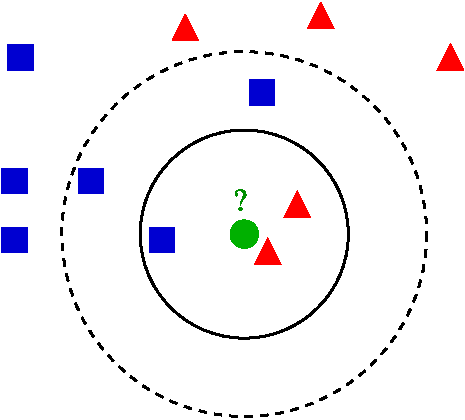
\includegraphics[width=0.4\textwidth]{images/KnnClassification}};
        \node (2) at (0.2, -1.3) {$k = 3$};
        \node (3) at (0.2, -2.6) {$k = 5$};
    \end{tikzpicture}
    \caption{Funcionamiento del algoritmo KNN \cite{knnalgorithm2010}}
    \label{fig:knn_clasification}
\end{figure}

En la Fig. \ref{fig:knn_clasification} se quiere clasificar el dato \textcolor{verdedato}{\Large$\bullet$}, una opción es usar múltiples valores de $k$ y con ello obtener diferentes resultados:
\begin{itemize}
    \item Asignando $k = 3$ sólo se tendrán en cuenta los 3 datos más próximos, que serán 2 de la clase \textcolor{rojodato}{\large$\blacktriangle$} y uno de la clase \textcolor{azuldato}{$\blacksquare$}. Con esto la clase que se asignará al dato \textcolor{verdedato}{\Large$\bullet$} será \textcolor{rojodato}{\large$\blacktriangle$}.
    \item Asignando $k = 5$ sólo se tendrán en cuenta los 5 datos más próximos, que serán 2 de la clase \textcolor{rojodato}{\large$\blacktriangle$} y tres de la clase \textcolor{azuldato}{$\blacksquare$}. Con esto la clase que se asignará al dato \textcolor{verdedato}{\Large$\bullet$} será \textcolor{azuldato}{$\blacksquare$}.
\end{itemize}

\subsubsection{Máquinas de vector soporte (SVM)}

Las máquinas de vector soporte son un conjunto de algoritmos de aprendizaje supervisado que se utilizan tanto para clasificación como para regresión, en este caso se analizará únicamente en clasificación.

Estos algoritmos toman los datos como puntos en un espacio $n-$dimensional. El objetivo es dividir estos datos mediante hiperplanos de forma que los puntos que contenidos en una región del espacio delimitada por los mismos hiperplanos sean una misma clase y que estén lo más separados posible. Esto se puede ver más fácil con un ejemplo.

En la Fig. \ref{fig:svm_separation} se puede ver como hay distintos hiperplanos ($\mathcal{H}_1, \mathcal{H}_2, \mathcal{H}_3$) que pueden dividir el espacio. 

\begin{itemize}
    \item $\mathcal{H}_1$ no divide de forma correcta todos los puntos de la entrada, puesto que hay puntos negros juntos con blancos.
    \item $\mathcal{H}_2$ sí que divide a todos los puntos en dos clases de la forma correcta, pero no están seraparas lo máximo posible de este hiperplano.
    \item $\mathcal{H}_3$ sí que cumple con las restricciones de división y distancia máxima.
\end{itemize}

\begin{figure}
    \centering
    \begin{tikzpicture}
        \node (1) {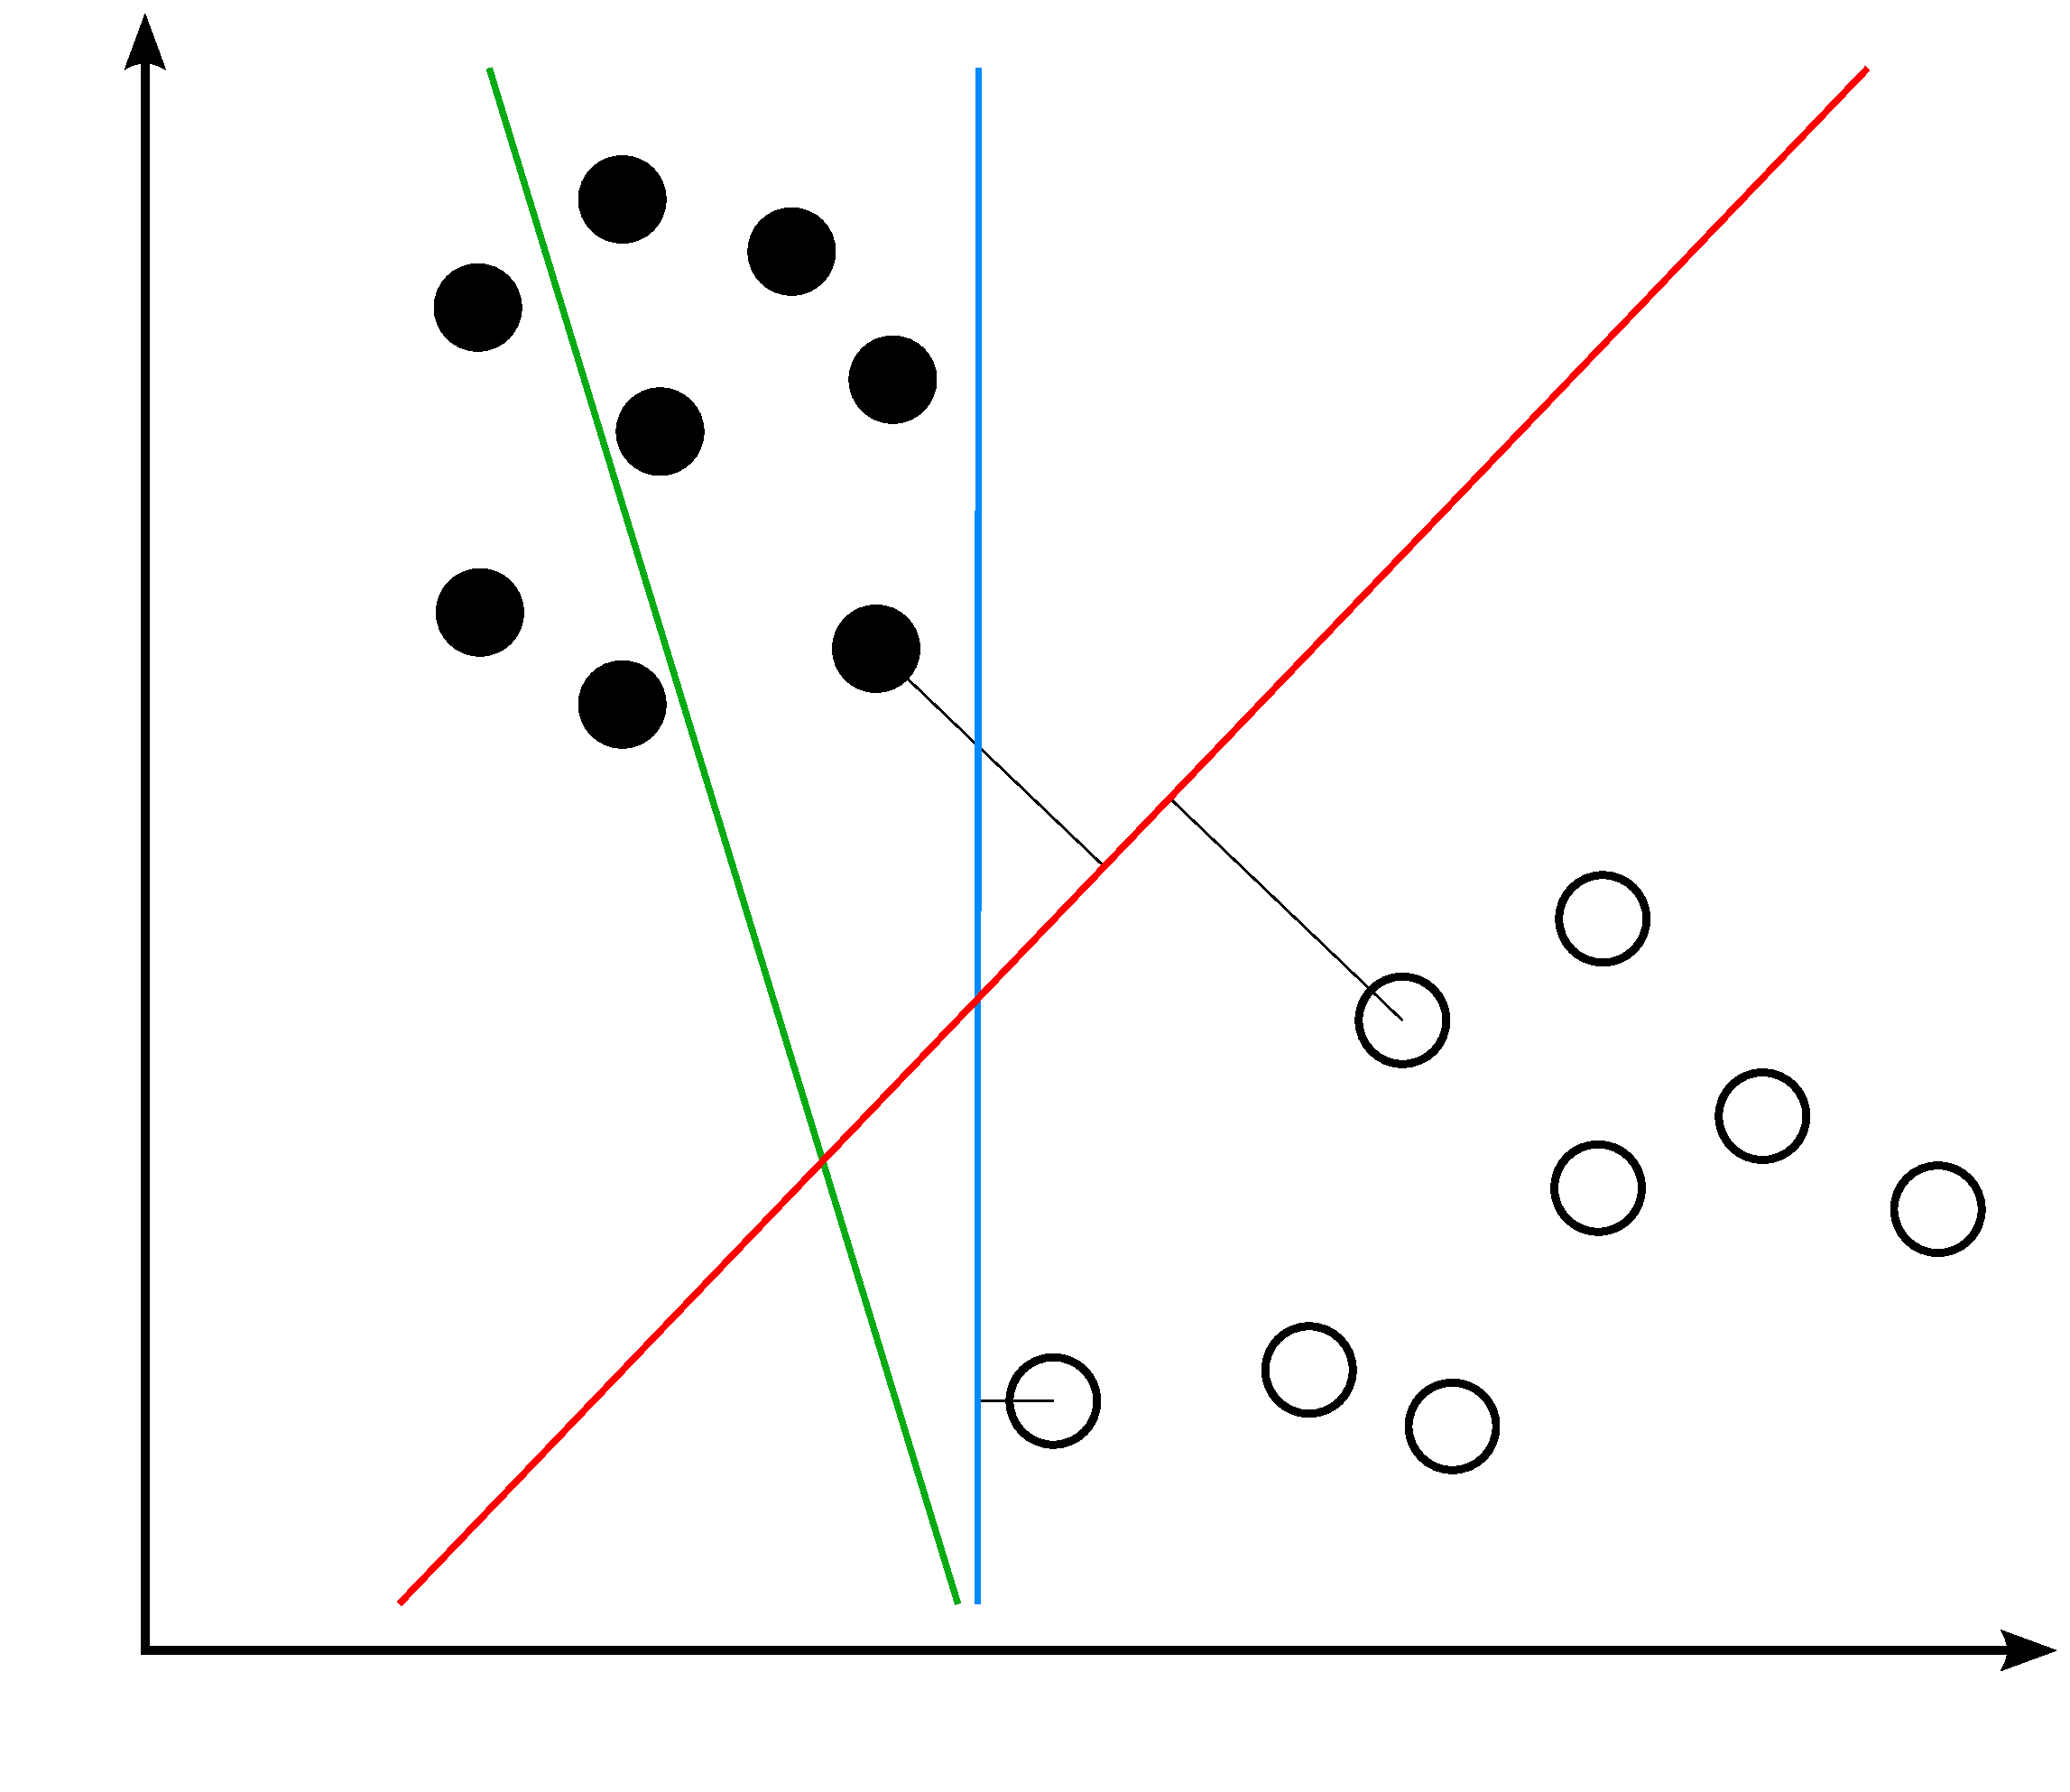
\includegraphics[width=0.4\textwidth]{images/svm_separation}};
        \node (2) at (2.7, -2.7) {$x_1$};
        \node (3) at (-3.2, 2.2) {$x_2$};
        \node (4) at (-2, 2.5) {\scriptsize $\mathcal{H}_1$};
        \node (5) at (-0.5, 2.5) {\scriptsize $\mathcal{H}_2$};
        \node (6) at (2, 2.5) {\scriptsize $\mathcal{H}_3$};
    \end{tikzpicture}
    \caption{Separación por hiperplanos SVM \cite{svmseparation2012}}
    \label{fig:svm_separation}
\end{figure}

En muchas ocasiones no se podrán dividir los conjuntos de forma correcta usando únicamente divisiones lineales del espacio, por ello, habrá que usar divisiones no lineales.

\section{Revisión bibliográfica}

En esta sección se realiza un estudio del estado del arte relativo a la aplicación de distintas técnicas que tengan como objetivo identificar a un dispositivo a través de la red independientemente de un identificador susceptible de ser identificado. Para estos cometidos son muy utilizados los algoritmos de aprendizaje automático o Machine Learning. 

Para comenzar la revisión bibliográfica, se analizará el trabajo desarrollado por Pascal Oser et al. \cite{oser2018identifying}. En este trabajo se desarrolla un sistema para identificar dispositivos entre un total de 562 en el centro del CERN. Para este cometido se tomas muestras periódicas de las marcas de tiempo (timestamps) contenidas en paquetes TCP que se envían y reciben de estos dispositivos.

De estas marcas se obtienen las variables que se usarán para entrenar los distintos modelos de machine learning. Las variables que obtiene son el incremento entre dos marcas consecutivas, el desbordamiento del contador de la marca de tiempo, la mediana de todas las marcas, etc.

Una variable interesante es la del desbordamiento del contador. En el RFC 1323 \cite{RFC1323} se define que el contador del timestamp (campo TSval) tiene una longitud de 4 bytes (32 bits), por lo tanto, el mayor valor que podrá tener asignado es $2^{32}$, puesto que es un entero sin signo. Se podría pensar que todos los dispositivos desbordan a la vez, pero cada fabricante establece el valor al que el contador se desborda. Esto está ilustrado en la Fig. \ref{fig:cern_ts_overflow} con dos ejemplos.

\begin{figure}
    \centering
    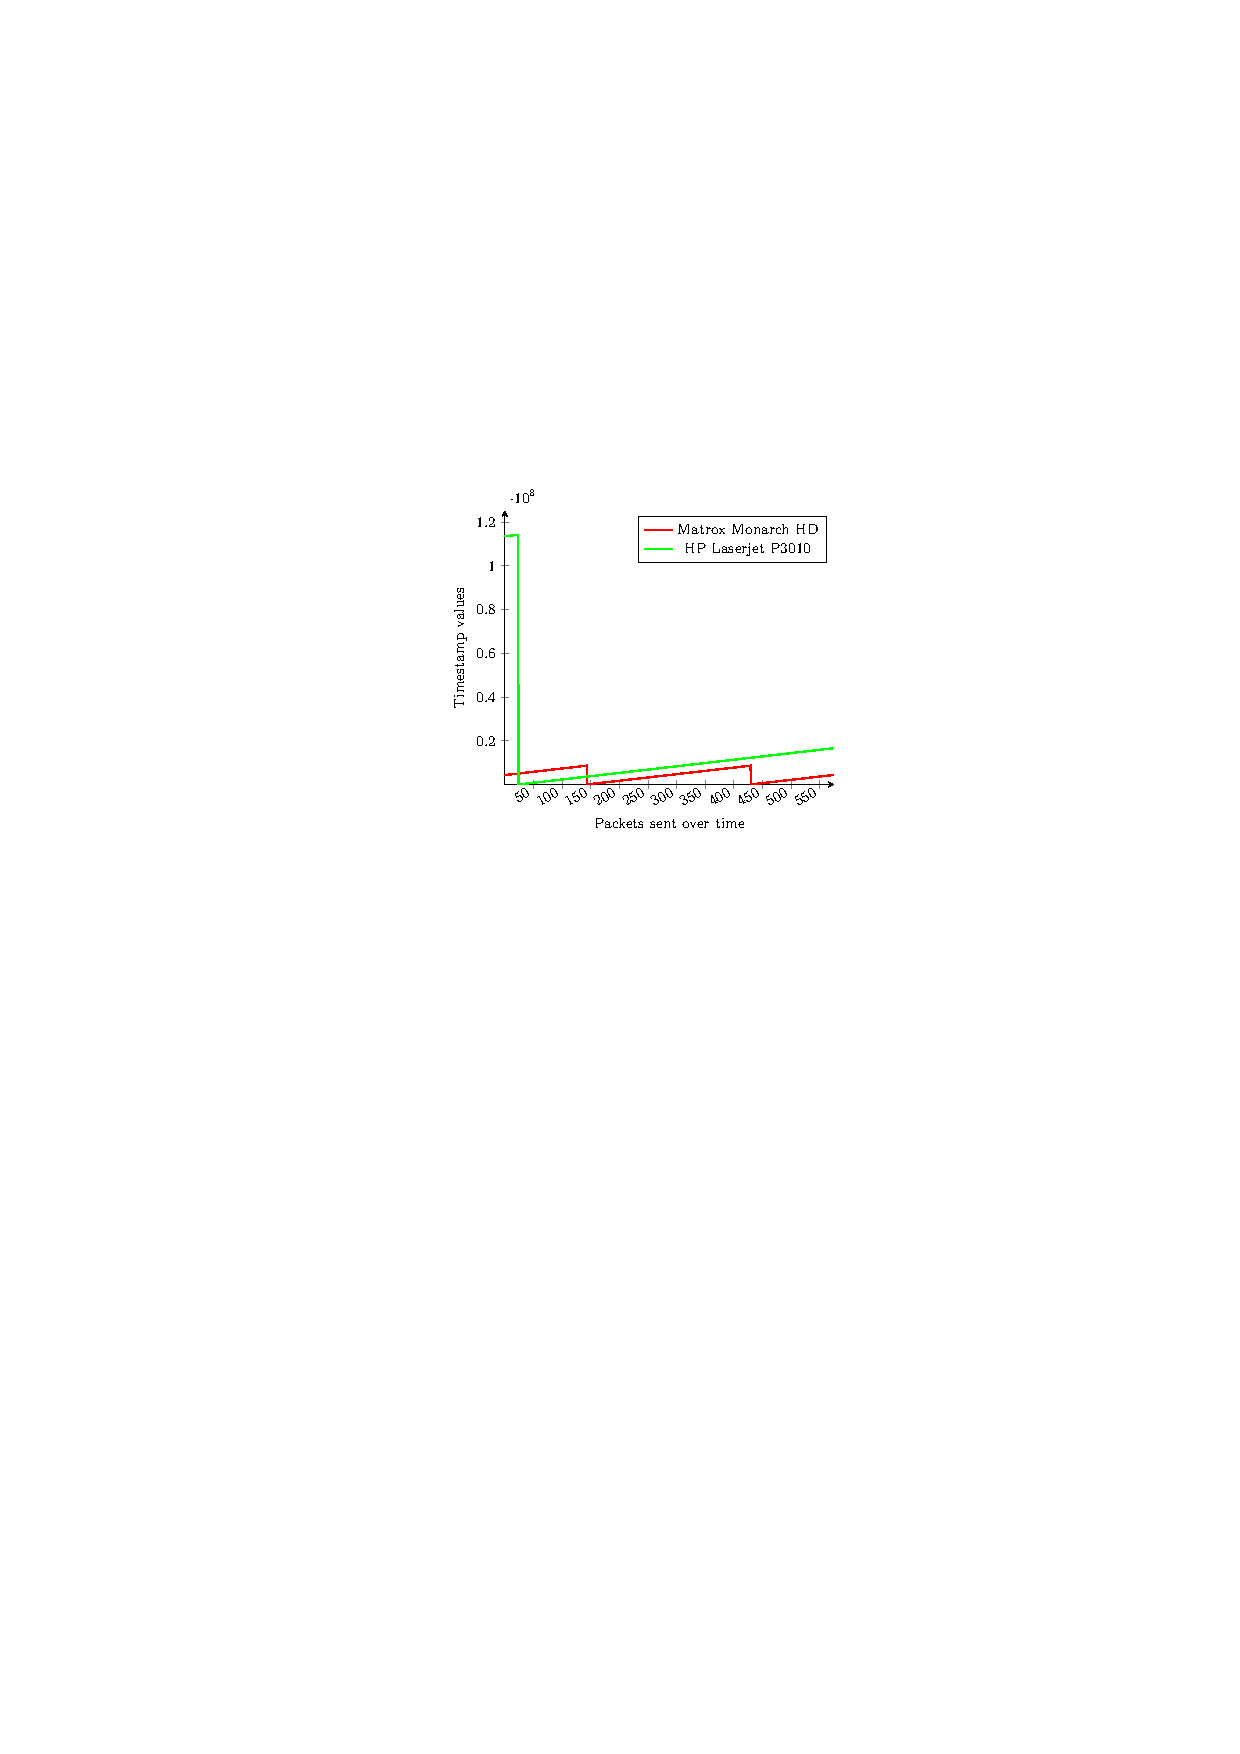
\includegraphics[width=0.45\textwidth]{images/CERN-timestamp_overflow}
    \caption{Desbordamiento del contador \cite{oser2018identifying}}
    \label{fig:cern_ts_overflow}
\end{figure}

Una vez tiene todas las variables registradas para todos los dispositivos, compara varios modelos de machine learning, para clasificar cada uno de los dispositivos. Los resultados que obtiene son de un accuracy del 99.22\% con MLP, un 99.14\% con SVM y por último 99.67\% con Random Forest.

Con estos datos decide quedarse con el modelo de Random Forest, el cual entrena con la totalidad de los datos de entrenamiento, obteniendo finalmente una precisión del 97.03\% y un accuracy del 99.76\%.

Otro trabajo relacionado con la temática ha sido desarrollado por Salma Abdalla Hamad et al. \cite{hamad2019iot}. En este trabajo se desarrolla un sistema que identifique a un dispositivo que quiere conectarse a la red y decida si se le permite realizar esta acción o se le deniega. Además este sistema comprobará periódicamente los dispositivos que están ya en la red para detectar comportamientos malintencionados. 

Este sistema (Fig. \ref{fig:diam_hamad}), una vez se tiene una traza del dispositivo que se quiere conectar por primera vez a la red, crea una huella del dispositivo que será analizada por un modelo (previamente entrenado) que lo clasificará como desconocido o no, en caso de que esté en una lista blanca. En caso de ser un dispositivo desconocido se le denegará el acceso a la red. Por contra, si está en la lista, se consultará una matriz de autorización (que contiene la confianza de ese dispositivo según sus vulnerabilidades) para saber que privilegios recibirá ese dispositivo. Con esto el dispositivo puede contectarse como un dispositivo ``confiable'', teniendo acceso a comunicarse con todos los dispositivos de la red, o por contra, de ``acceso restringido'' donde solo podrá comunicarse con dispositivos de ese mismo nivel de acceso.

\begin{figure}
    \centering
    \resizebox{0.6\textwidth}{!}{
        \begin{tikzpicture}
    \node[draw, text width = 2cm, align = center, minimum width = 2cm, fill = blancodiagrama, execute at begin node=\setlength{\baselineskip}{1em}] (1) {\footnotesize Sequence Capture};
    \node (2) [left = 3cm of 1] {};
    \node[draw, rounded corners, fill = azuldiagrama] (3) [below = of 1] {\footnotesize Finger Print};
    \node[draw, diamond, aspect = 2, fill = azuldiagrama] (4) [below = of 3] {\footnotesize Classifier};
    \node[draw, cylinder, rotate = 90, fill = verdediagrama, minimum height = 0.5cm, minimum width = 0.5cm, scale = 0.5] (5) at (-0.9,-3.85) {};
    \node[draw, rounded corners, fill = azuldiagrama] (6) [below = of 4] {\footnotesize Zoning};
    \node (7) [left = 3cm of 6] {};
    \node (8) [below = of 6] {};
    \node[draw, fill = verdediagrama] (9) [left = of 8] {\footnotesize Trusted};
    \node[draw, fill = naranjadiagrama] (10) [right = of 8] {\footnotesize Restricted};
    \node[draw, text width = 2cm, align = center, minimum width = 2cm, fill = blancodiagrama, execute at begin node=\setlength{\baselineskip}{1em}] (11) [below = of 8] {\footnotesize Random Capture};
    \node[draw, rounded corners, fill = azuldiagrama] (12) [below = of 11] {\footnotesize Finger Print};
    \node[draw, diamond, aspect = 2, fill = azuldiagrama] (13) [below = of 12] {\footnotesize Classifier};
    \node[draw, cylinder, rotate = 90, fill = verdediagrama, minimum height = 0.5cm, minimum width = 0.5cm, scale = 0.5] (14) at (-0.9,-12.73) {};
    \node[draw, ellipse, minimum height = 1.5cm, fill = verdediagrama] (15) [left = of 13] {\footnotesize Match};
    \node[draw, fill = rojodiagrama] (16) [left = 2.5cm of 9] {\footnotesize Rejected};
    \node[draw, fill = rojodiagrama] (17) [right = 2.5cm of 10] {\footnotesize Quarantine};
    \node (18) [above right = 4.7cm of 13] {};
    \node (19) [below right = 0.7cm of 13] {};
    
    \draw (2) -- (1) node [midway, above, text width = 2.5cm, align = center] {\footnotesize Unseen Device Network Traces};
    \draw (2) -- (1) node [midway, below, text width = 2.5cm, align = center] {\footnotesize 010111000011001};
    \draw (1) -- (3);
    \draw (3) -- (4);
    \draw (4.west) -| (16.north) node [pos=0.25, above] {\footnotesize Unknown Device};
    \draw (4) -- (6);
    \draw (7) -- (6) node [above, midway] {\scriptsize Authorisation Matrix};
    \draw (6) -- (9);
    \draw (6) -- (10);
    \draw (9) -- (11);
    \draw (10) -- (11);
    \draw (11) -- (12);
    \draw (12) -- (13);
    \draw (15) -- (13);
    \draw (13) -| (18.center) node [pos=0.25, above] {\footnotesize Mis-Classified} |- (6);
    \draw (13) |- (19.center) -| (17) node [pos=0.17, above] {\footnotesize Suspicious/Mis-Behaving};
\end{tikzpicture}
    }
    \caption{Modelo del sistema de identificación \cite{hamad2019iot}}
    \label{fig:diam_hamad}
\end{figure}

Para los dispositivos que ya están conectados a la red, se toma una muestra aleatoria que comprobará si se han clasificado de forma correcta. En el caso de que se haya clasificado mal pero siga estando en la lista blanca se actualizará su matriz de autorización. Por otra parte, en caso de que no esté en dicha lista se pondrá en cuarentena para ser analizado más adelante.

Las huellas de los dispositivos se obtienen del payload de los mensajes enviados por ese dispositivo. De ellos se obtienen 67 características como el tamaño del paquete Ethernet, el tamaño de las cabeceras, la IP de destino, el TTL, etc.

Con estas huellas entrena distintos modelos como son AdaBoost, LDA, KNN, Árboles de decisión, Naive Bayes, SVM, Random Forest y GBoost. Obtuvo un accuracy final del 89\%.

El siguiente artículo que se analizará es el realizado por Ahmet Aksoy et al. \cite{aksoy2019automated}. Este trabajo diseña un sistema (llamado SysID) que es capaz de identificar dispositivos a través del tráfico de red. 

Este sistema únicamente necesita un paquete de red para identificar el dispositivo. Dado un paquete de la traza se seleccionan $n$ cabeceras del paquete mediante un algoritmo genético, que implementa una función fitness (Eq. \ref{eq:aksoy_fit}) que trata de reducir este número de cabeceras. 

\begin{equation}
    Fitness = 0.9 \cdot Accuracy + 0.1 \cdot \left( 1 - \frac{\lvert SelectedFeatures \rvert - 1}{\lvert AllFeatures \rvert - 1} \right)
    \label{eq:aksoy_fit}
\end{equation}
donde $n = \lvert SelectedFeatures \rvert$ y $Accuracy$ es el resultado que se obtiene del modelo de machine learning entrenado con esas cabeceras.

Las trazas que se han usado para clasificar estos dispositivos provienen de una base de datos de otro artículo \cite{miettinen2017iot}, de donde se obtienen 20 medidas de 23 dispositivos IoT.

Para la clasificación se han usado diferentes algoritmos de la herramienta WEKA \cite{hall2009weka} como son tablas de decisión, árboles de decisión J48, OneR y PART. Se decide usar una clasificación en dos niveles (Fig. \ref{fig:askoy_classifier}), se clasifican primero entre su proveedor o el propio dispositivo, dependiendo de si hay más de un mismo dispositivo del mismo proveedor. Después se clasifican los dispositivos del mismo proveedor entre sí. Este esquema ayuda a tener mejores resultados pues cada proveedor puede ser identificado de mejor forma por un algoritmo distinto.

Los resultados que obtiene son de un 82\% de accuracy promedio entre todos los clasificadores de cada proveedor. Los valores individuales están entre el 42.2\% y el 100\%.

\begin{figure}
    \centering
    \resizebox{0.6\textwidth}{!}{
        \begin{tikzpicture}
    \node[draw, fill = azulclasificador, minimum width = 4.5cm] (0) {Hue Classifier};
    \node[draw, fill = azulclasificador, minimum width = 4.5cm] (1) [left = of 0] {Device Genre Classifier};
    \node[draw, fill = azulclasificador, minimum width = 4.5cm] (2) [above = 0.4cm of 0] {EdimaxPlug Classifier};
    \node[draw, fill = azulclasificador, minimum width = 4.5cm] (3) [above = 0.4cm of 2] {D-Link Classifier};
    \node[draw, fill = azulclasificador, minimum width = 4.5cm] (4) [below = 0.4cm of 0] {TP-Link Classifier};
    \node[draw, fill = azulclasificador, minimum width = 4.5cm] (5) [below = 0.4cm of 4] {Smarter Classifier};
    \node[draw, diamond, shape aspect = 2, fill = rojoclasificador] (6) [below = 0.4cm of 5] {Result};
    \node[draw, diamond, shape aspect = 2, fill = rojoclasificador] (7) [right = of 0] {Result};
    \node[draw, tape, tape bend top = none, tape bend height = 6pt, text width = 2.3cm, align = center, fill = verdeclasificador] (8) [above = 1.72cm of 1.west, anchor = west] {Arff file \\ (All devices)};
    
    \draw (1) -- (0);
    \draw (1.north) to [bend left = 18] (2.west);
    \draw (1.north) to [bend left] (3.west);
    \draw (1.south) to [bend right = 18] (4.west);
    \draw (1.south) to [bend right] (5.west);
    \draw (1.south) to [bend right] (6.west);
    
    \draw (0) -- (7);
    \draw (3.east) to [bend left] (7.north); 
    \draw (2.east) to [bend left] (7.north west); 
    \draw (4.east) to [bend right] (7.south west); 
    \draw (5.east) to [bend right] (7.south); 
    
    \draw (8) -- (8 |- 1.north);
\end{tikzpicture}
    }
    \caption{Clasificador de dos niveles \cite{aksoy2019automated}}
    \label{fig:askoy_classifier}
\end{figure}

El siguiente trabajo que se verá es el realizado por Hossein Jafari et al. \cite{jafari2018iot}. En este artículo no se utilizan paquetes de la capa de red o transporte, sino de la capa física. Para realizar esta labor se obtendrá la huella de cada dispositivo mediante radio frecuencias, por esta razón, este estudio sólo se centrará en conexiones inalámbricas, en este caso 6 dispositivos ZigBee \cite{gislason2008zigbee}.

Para cada uno de los dispositivos se realiza una captura de 5 minutos. Esta captura será del SNR en 5 niveles distintos, con lo que se obtiene \SI{10}{\giga\byte} por dispositivo y nivel de SNR, lo que en total serían \SI{300}{\giga\byte} de datos.

A continuación procede a entrenar tres modelos de deep learning, DNN, CNN y LSTM (los tres modelos pertenecen a la librería \texttt{TensorFlow} programada para Python \cite{tensorflow2015-whitepaper}), con los que obtiene unos resultados de 96.3\%, 94.7\% y 76\% respectivamente.

Fabian Lanze et al. \cite{lanze2012clock} han desarrollado un trabajo en el que crean un sistema de identificación de dispositivos basado en el clock skew. Su objetivo es generar huellas para cada punto de acceso, de forma que si un dispositivo pueda saber si ese punto de acceso es legítimo, o por contra si puede ser un potencial atacante.

Lo primero que hacen es definir el skew de un reloj como la primera derivada del offset de dicho reloj. De forma práctica usarán la desviación que almacena el demonio del servicio NTP para aproximar el skew del dispositivo conectado al punto de acceso. Usará conexión inalámbrica y recogerá hasta 6000 paquetes por dispositivo en cada muestra (10 minutos). Si en una muestra no se alcanzan los 500 paquetes, por problemas de conexión o cualquier otro motivo, esa muestra se elimina. Con este proceso se consiguen medir 388 puntos de acceso. 

Finalmente, trata de generar una huella para cada punto de acceso de forma estadística, basándose sobre todo en la distribución del clock skew. Como resultado obtiene que su método no es suficientemente preciso y que muchos dispositivos presentan una huella similar, por lo tanto, concluye que no es posible identificarlos únicamente de esta forma.

En el trabajo desarrollado por Yair Meidan et al. \cite{meidan2017profiliot} se desarrolla un sistema que es capaz de identificar dispositivos IoT a través de su tráfico de red. Las pruebas se realizan con trazas sobre conexión inalámbrica y tanto con dispositivos IoT como con PCs, smartphones, etc. 

De estas trazas se centran específicamente en las sesiones TCP, donde cada una se representa como un conjunto de características de cada paquete.

Primeramente, ejecutan un clasificador binario con el que obtienen la probabilidad de que un dispositivo sea IoT, usando solo información de una sesión TCP de cada dispositivo. En este apartado obtienen un \SI{100}{\percent} de acierto.

Por último, entrenan distintos modelos de clasificación (GBM, Random Forest, XGBoost), únicamente sobre los dispositivos previamente etiquetados como IoT, obteniendo finalmente un resultado de un \SI{99.281}{\percent} de accuracy en la identificación del modelo y marca de cada uno de ellos.

Como último artículo se analizará la propuesta realizada por Loh Chin Choong Desmond et al. \cite{desmond2008identifying}. En este trabajo han construido un sistema de identificación de dispositivos basado en los mensajes \textit{probe request} de los distintos dispositivos. Para ello, distinguirán como dispositivos distintos las distintas combinaciones de la tupla: $\langle$``Machine'', ``Wireless Network Interface Card (NIC) Driver'', ``Operating System''$\rangle$.

A continuación, comprueban que en el tiempo de emisión de estos mensajes se ven varios comportamientos que se repiten. Luego, observan que la latencia entre ráfagas de estos mensajes también presenta estos comportamientos distintivos. Con estas latencias son con las que entrenarán un modelo que sea capaz de distinguir los dispositivos.

El modelo que eligen se basa en aprendizaje no supervisado, Maximum Variance Clustering \cite{veenman2002maximum}. Este modelo es similar al algoritmo de $k$-medias, la distinción es que $k$-medias necesita conocer previamente el número de clústeres $k$ previamente, mientras que Maximum Variance Clustering necesita conocer la varianza máxima dentro de un clúster $\sigma^2_{max}$. Con este algoritmo obtienen unos resultados de accuracy entre el \SI{70}{\percent} y el \SI{80}{\percent}.


\subsection{Resultados de la revisión bibliográfica}

Por último se realizará un resumen en forma de tabla de los artículos que han sido revisados. 

\begin{table}
    \centering
    \resizebox{\textwidth}{!}{
        \begin{tabular}{C{0.12\textwidth}C{0.15\textwidth}C{0.15\textwidth}C{0.15\textwidth}C{0.14\textwidth}C{0.2\textwidth}C{0.24\textwidth}}
            \toprule
            Referencia & Tipo de identificación & Fuente de los datos & Método de clasificación & Tipo de aprendizaje & Algoritmos usados & Resultados \\
            \midrule
            \cite{oser2018identifying} & Tipo de dispositivo & Cabeceras TCP & Machine Learning & Supervisado & MLP, SVM, Random Forest & 99.76\% de accuracy y 97.03\% de precisión \\
            \addlinespace\addlinespace
            \cite{hamad2019iot} & Individual & Característi-cas del payload & Machine Learning & Supervisado & AdaBoost, LDA, KNN, Árboles de decisión, Naive Bayes, SVM, Random Forest y GBoost & 89\% de accuracy \\
            \addlinespace\addlinespace
            \cite{aksoy2019automated} & Tipo y modelo del dispositivo & Cabereceras TCP & Machine Learning & Supervisado & Tablas de decisión, Árboles de decisión J48, OneR y PART & Entre 42.2\% y 100\% de accuracy, con un promedio de 82\% \\
            \addlinespace\addlinespace
            \cite{jafari2018iot} & Individual & Radio frecuencias & Machine Learning & Supervisado & DNN, CNN y LSTM & 96.3\% de accuracy en DNN, 94.7\% de accuracy en CNN y 76\% de accuracy en LSTM \\
            \addlinespace\addlinespace
            \cite{lanze2012clock} & Modelo del dispositivo & Registros NTP & Estadístico & - & - & Inconcluyentes \\
            \addlinespace\addlinespace
            \cite{meidan2017profiliot} & Tipo y modelo & Sesiones TCP & Machine Learning & Supervisado & GBM, Random Forest y XGBoost & \SI{99.281}{\percent} de accuracy \\
            \addlinespace\addlinespace
            \cite{desmond2008identifying} & Individual & Mensajes \textit{probe request} & Machine Learning & No supervisado & Maximum Variance Clustering & Entre un 70\% y 80\% de accuracy\\
            \addlinespace\addlinespace
            Este trabajo & Individual & Ciclos de CPU & Machine Learning & Supervisado y No supervisado & Random Forest, MLP, Naive Bayes, KNN, Árboles de decisón, SVM-Linear, LOF, OC-SVM, Isolation Forest & 99.38\% de Accuracy, 99.39\% de Recall y 99.38\% de $f$-score\\
            \bottomrule
        \end{tabular}
    }
    \caption{Resultados en el estado del arte}
    \label{tab:art_results}
\end{table}




% Análisis de objetivos y metodología 
%!TEX root = TFG.tex

\lstset{frame=single,basicstyle=\ttfamily\small}

\chapter{Análisis de objetivos y metodología} \label{chap:meto}

En esta sección se analizarán los objetivos del trabajo y se realizará un análisis sobre las decisiones tomadas en el proceso de identificar dispositivos.

\section{Análisis de objetivos}

El principal objetivo de este proyecto es conseguir identificar dispositivos idénticos. La solución que se propone es capaz de identificar los patrones relativos a la desviación de sus relojes internos y usarlos para reconocer a cada dispositivo mediante un modelo de Machine Learning. Para lograr dicho objetivo han sido establecidas diversas metas intermedias:

\begin{itemize}
    \item Usar lo visto en el estado del arte, para conocer y seleccionar los desafíos de este proyecto.
    \item Conseguir un registro de los relojes internos de cada uno de los dispositivos que se van a participar en el análisis. Para lo que definiremos una estructura cliente-servidor que recogerá un registro de los datos.
    \item Generar una huella estadística de estos registros. Para desarrollar este objetivo se hace uso de una ventana deslizante que permite agrupar los datos y extraer estadísticas comunes.
    \item Analizar distintas propuestas de algoritmos de Machine Learning que sean capaces de tomar como entrada las huellas estadísticas y, con ellas, identificar a cada dispositivo.
\end{itemize}

\section{Metodología de trabajo}

Para poder alcanzar los objetivos propuestos, se presenta una metodología de trabajo.

\begin{enumerate}
    \item \textbf{Revisión bibliográfica}. Revisión de los trabajos relacionados con el tema de este trabajo. En concreto, se busca comprender cómo obtienen sus datos y su método de clasificación de dispositivos.
    \item \textbf{Recolección de los datos}. Generación de un dataset que contiene las marcas de tiempo tanto del dispositivo de referencia como del que se encuentra bajo análisis. Este proceso se realiza por cada dispositivo a analizar.
    \item \textbf{Generación de huella estadística}. Por cada dispositivo se hace uso de una ventana deslizante que agrupa los datos en grupos de $n$ muestras. De cada grupo se obtienen un conjunto de variables estadísticas que son etiquetadas con el dispositivo del que se han obtenido.
    \item \textbf{Búsqueda de variables correlacionadas}. Se realiza un test de correlación a los datos con el fin de reducir la dimensionalidad de los mismos. Las variables correlacionadas no aportan información y por ello han de ser eliminadas.
    \item \textbf{Particionamiento del conjunto de datos}. Con el fin de entrenar algoritmos de Machine Learning, se divide el conjunto de datos en dos de menor tamaño (entrenamiento y test).
    \item \textbf{Ajuste de hiperparámetros}. Para decidir cuál de los algoritmos es mejor para clasificar los datos de este trabajo se comparan distintos algoritmos de Machine Learning. Estos algoritmos han de ser ajustados correctamente para obtener los mejores resultados. Para realizar este ajuste se realiza una partición similar a la realizada con el conjunto de todos los datos, pero con un conjunto reducido de forma que los entrenamientos duren menos tiempo.
    \item \textbf{Evaluación de los distintos modelos}. Una vez entrenados todos los algoritmos que se quieren comparar, se comparan sus resultados identificando dispositivos para elegir al mejor candidato.
    \item \textbf{Entrenamiento del modelo final}. Decididos el algoritmo que se va a usar y sus hiperparámetros, se realiza un entrenamiento final con el conjunto completo de los datos de entrenamiento.
    \item \textbf{Evaluación del modelo final}. Análisis de los resultados finales obtenidos.
\end{enumerate}


% Diseño y resolución
%!TEX root = TFG.tex

\chapter{Diseño y resolución} \label{chap:diseno}

En este capítulo se realiza la descripción de los experimentos realizados, su análisis y la búsqueda de un modelo de Machine Learning, así como los resultados finales del trabajo.

En este trabajo se usará una topología de red como la que ilustra la Fig. \ref{fig:top}. En dicha topología se puede ver que tenemos un observador (modelo RockPro64) y 5 dispositivos a analizar (Raspberry Pi 4 Model B).

\begin{figure}
    \centering
    \resizebox{0.5\textwidth}{!}{
        \begin{tikzpicture}
    \node (1) {
\includegraphics{cisco_icons/cloud}};
    \node (2) [below = of 1] {
\includegraphics{cisco_icons/router}};
    \node (3) [below = of 2] {$\substack{
\includegraphics{cisco_icons/pc} \\ \text{Observador}}$};
    \node (aux) [below =0.4cm of 3] {};
    \node (4) [below = of aux] {$\substack{
\includegraphics{cisco_icons/pc} \\ \text{Disp. 3}}$};
    \node (5) [left = of 4] {$\substack{
\includegraphics{cisco_icons/pc} \\ \text{Disp. 2}}$};
    \node (6) [left = of 5] {$\substack{
\includegraphics{cisco_icons/pc} \\ \text{Disp. 1}}$};
    \node (7) [right = of 4] {$\substack{
\includegraphics{cisco_icons/pc} \\ \text{Disp. 4}}$};
    \node (8) [right = of 7] {$\substack{
\includegraphics{cisco_icons/pc} \\ \text{Disp. 5}}$};
    \node (text) {Internet};
    \draw[-] (1) -- (2); 
    \draw[-] (2) -- (3);
    \draw[-] (3) -- (4);
    \draw[-] (aux.center) -| (6);
    \draw[-] (aux.center) -| (5);
    \draw[-] (aux.center) -| (7);
    \draw[-] (aux.center) -| (8);
\end{tikzpicture}
    }
    \caption{Topología de la red}
    \label{fig:top}
\end{figure}

La idea es mandar mensajes desde el observador a cada uno de los dispositivos y que cada uno de los dispositivos conteste a esos mensajes y obteniendo así una marca de tiempo de ese dispositivo.

\section{Elección del protocolo}

Las opciones barajadas han sido TCP e ICMP. En un principio se pensaba usar las marcas de tiempo contenidas en las cabeceras de estos protocolos, pero esta idea se descartó puesto que únicamente permitían obtener los tiempos en milisegundos. El objetivo era obtener los tiempos en nanosegundos por tanto, se enviaron los datos en el cuerpo del paquete que no tiene una limitación tan corta de espacio. 

Con el fin de mantener la conexión persistente en toda la muestra se escogió el protocolo TCP, ya que una vez establecida la conexión se mantendrá hasta el final.

\section{Obtención de datos}

Para obtener los datos se usará una estructura cliente-servidor. Los dispositivos a analizar serán los que tomen el rol de servidores y el observador será el cliente.

Con esta idea en mente se crea un programa servidor que escuche a cualquier dirección IP en un determinado puerto y responda con una marca de tiempo en nanosegundos. Este programa se ejecutará en cada uno de los dispositivos bajo análisis.

A la hora de capturar los datos se usó un reloj interno que no debería sufrir alteraciones que disminuyeran su valor (\texttt{steady\_clock}\cite{steadyclockcpp}).

Una vez los dispositivos estén todos escuchando, el observador ejecutará un programa cliente que es el que se encargará de enviar los mensajes al servidor correspondiente. Este programa guarda una marca de tiempo al comienzo de la ejecución $t_{start}$, que será nuestro punto de referencia. Después mandará $n$ mensajes equiespaciados en intervalos de 1 segundo.

En cada ejecución del bucle se obtendrá una marca de tiempo en el observador $t_i$, y una marca de tiempo del dispositivo $t'_i$. Con esto se consiguen tener varios datos:
\begin{itemize}
    \item La marca de tiempo relativa a cada mensaje desde el inicio, $t_i - t_{start}$. Teóricamente debería de dar valores exactos, ya que se manda un mensaje cada segundo, pero existe cierto retraso.
    \item La marca de tiempo absoluta del observador $t_i$.
    \item La marca de tiempo absoluta del dispositivo $t'_i$.
    \item La desviación del reloj del dispositivo respecto al del observador, $t_i - t'_i$.
\end{itemize}

Un ejemplo de como se guardan estos datos se puede ver en la Tabla \ref{tab:trace_example}.
\begin{table}
    \centering
    \resizebox{0.75\textwidth}{!}{
    \begin{tabular}{ccccc}
        \toprule
        \texttt{time} & \texttt{TSrock} & \texttt{TSrasp} & \texttt{offset} & \texttt{device} \\
        \midrule
        292 & 119238112796030 & 104592709716803 & -14645403079227 & 192.168.1.111 \\
        1001191222 & 119239113986960 & 104593710167425 & -14645403819535 & 192.168.1.111 \\
        2001485862 & 119240114281600 & 104594710453699 & -14645403827901 & 192.168.1.111 \\
        \vdots & \vdots & \vdots & \vdots & \vdots \\
        \bottomrule
    \end{tabular}
    }
    \caption{Ejemplo de los datos obtenidos de cada dispositivo}
    \label{tab:trace_example}
\end{table}

Este proceso se realizará para cada dispositivo tanto en una muestra secuencial, como en una muestra en paralelo.


\section{Análisis de los datos}

En esta sección se estudiará el incremento de la desviación del reloj en cada una de las muestras, así como la desviación acumulada en cada punto.

\subsection{Experimento 1: Muestra secuencial}

En este primer experimento se ha tomado una muestra de \SI{7200}{} segundos, es decir, \SI{2}{} horas por dispositivo, lo que en total suman \SI{10}{} horas de muestras.

En la Fig. \ref{fig:off_acu_secuencial} se muestra la desviación (offset) acumulada en cada dispositivo durante esas \SI{2}{} horas.

\begin{figure}
    \centering
    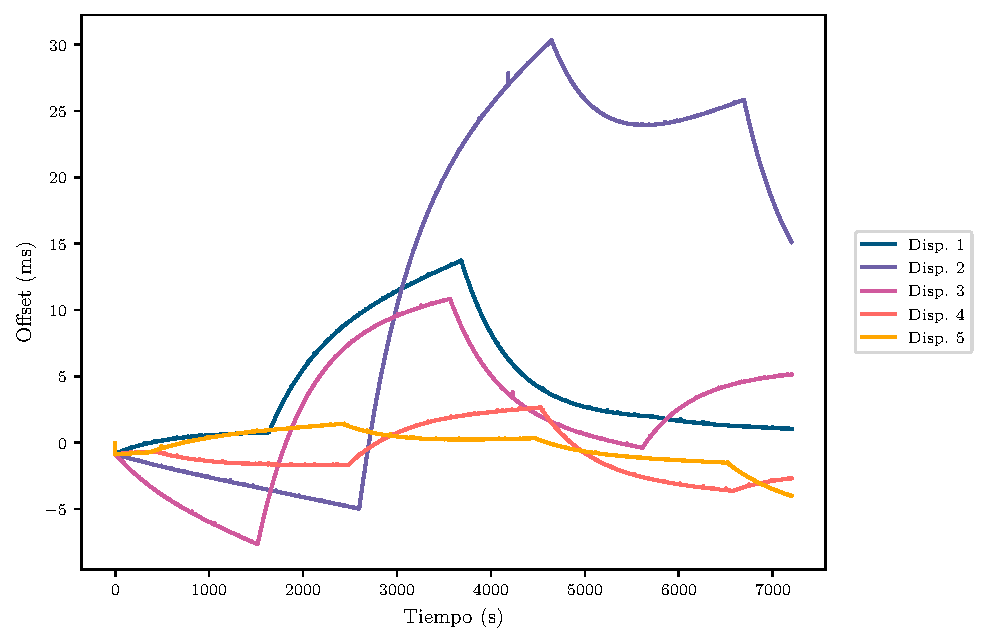
\includegraphics[scale=0.65]{../Python/plots/individual/offset_plot}
    \caption{Offset acumulado muestra secuencial}
    \label{fig:off_acu_secuencial}
\end{figure}

Como se puede ver hay 2 tipos de comportamiento. Los dispositivos 1, 2 y 3 se mantienen monótonos al comienzo para después incrementar mucho su desviación. Por contra los dispositivos 4 y 5 se mantienen sin grandes cambios en toda la muestra. Esto se puede ver más claramente en la Fig. \ref{fig:off_acu_secuencial_diffs}.

\begin{figure}
    \centering
    \subfloat[Dispositivos 1, 2 y 3]{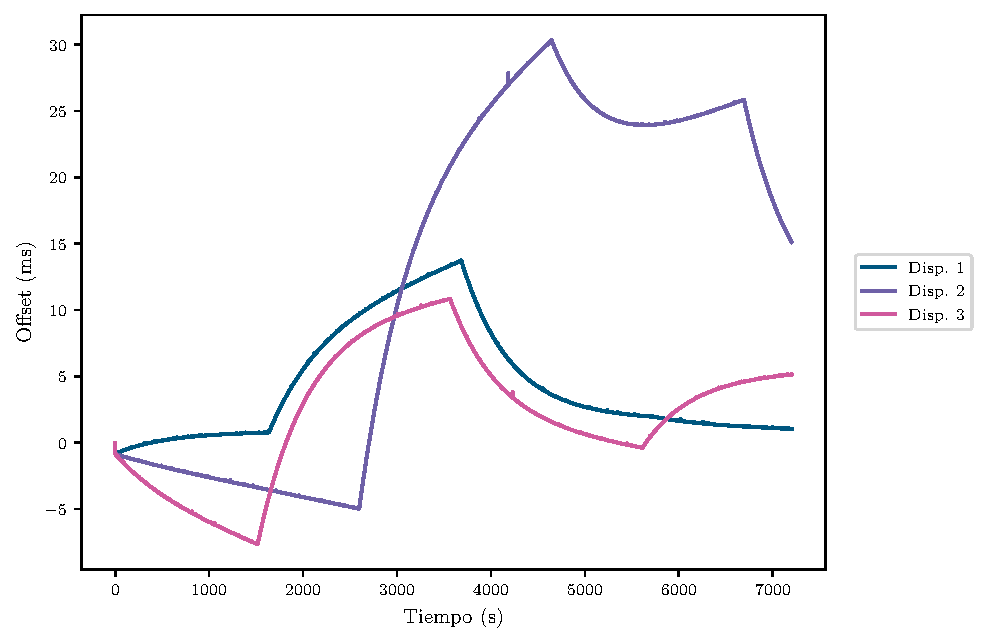
\includegraphics[width=0.4\textwidth]{../Python/plots/individual/offset_plot_123}}
    \quad
    \subfloat[Dispositivos 4 y 5]{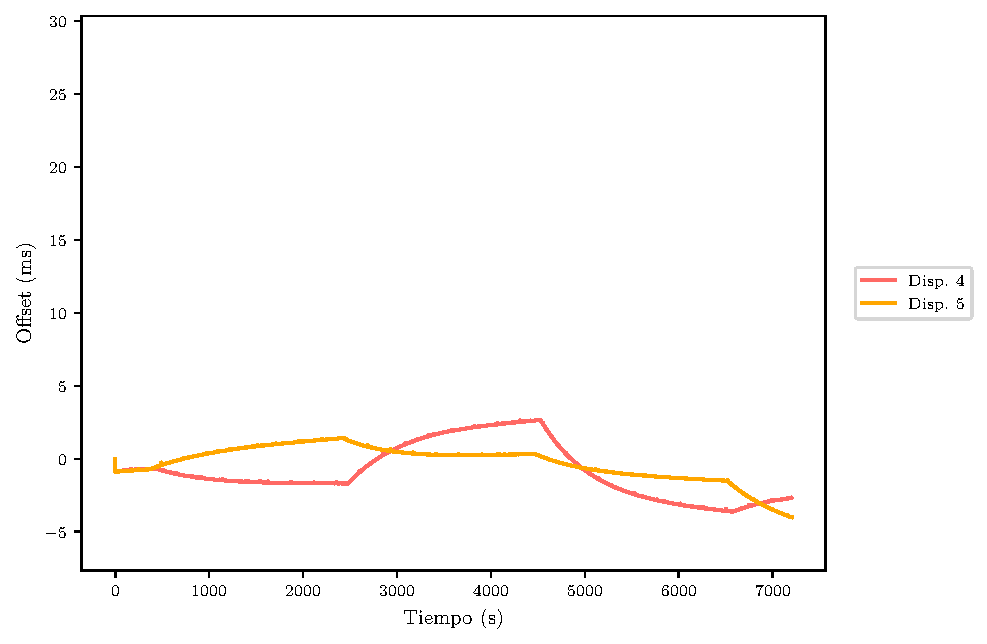
\includegraphics[width=0.4\textwidth]{../Python/plots/individual/offset_plot_45}}
    \caption{Diferencias entre offsets de dispositivos}
    \label{fig:off_acu_secuencial_diffs}
\end{figure}

Lo que interesa al final es obtener una forma de distinguir estadísticamente los datos, para ello se genera un gráfico que muestre entre que valores se mueven estos datos en cada dispositivo, en definitiva, se puede ver con un diagrama de cajas (Fig. \ref{fig:box_secuencial}). Se han eliminado los valores atípicos ya que a tan pequeña escala no dejan ver los verdaderos resultados.

\begin{figure}
    \centering
    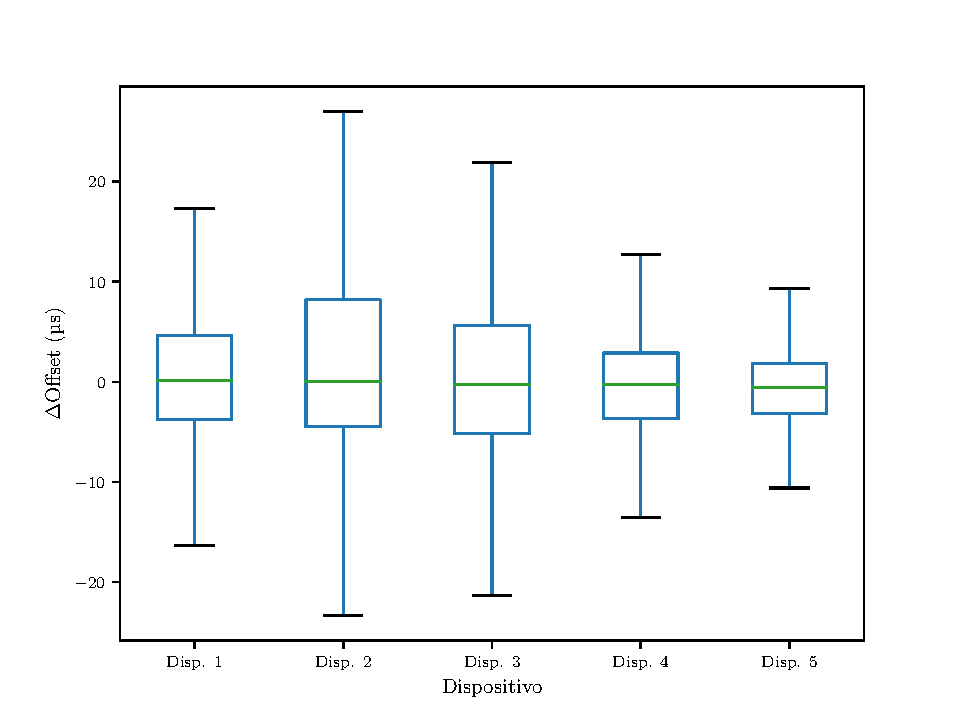
\includegraphics[scale=0.7]{../Python/plots/individual/boxplot_no_out}
    \caption{Diagrama de cajas muestra secuencial}
    \label{fig:box_secuencial}
\end{figure}

Este diagrama ilustra lo comentado anteriormente. Los dispositivos 4 y 5 son los que menos varían, esto se puede ver en que las cajas son pequeñas y la mediana está centrada entre los cuartiles (Q1 y Q3). 

En los otros 3 dispositivos se observa como entre la mediana y el tercer cuartil hay más espacio que entre la mediana y el primer cuartil. Esto se debe a que tienen muchos incrementos grandes, por eso crecen tan bruscamente.

Con esto se tiene una idea de los dispositivos son distinguibles estadísticamente, lo que confirma que se podrá entrenar un modelo que los identifique.

\iffalse
Por último se obtienen las variables estadísticas que podrán ser usadas para entrenar los modelos (Tabla \ref{tab:stats_sec}). 

\begin{table}
    \centering
    \resizebox{0.85\textwidth}{!}{
        \begin{tabular}{c|c|c|c|c|c|c|c|c|c|c|c}
             & Sum & Mean & Median & Mode & Std & IQR & Kurtosis & Skew & Max & Min & Device \\
             \hline\hline
            1 & 161935.0 & 2698.9166666666665 & 2368.0 & -10638.0 & 4811.992019561929 & 4723.75 & 1.9261137847830017 & 0.393744697396757 & 16643.0 & -10638.0 & Disp. 1 \\
            2 & -133618.0 & -2226.9666666666667 & -2069.0 & -14962.0 & 4940.972387543091 & 3037.75 & 3.06918010272503 & 0.3990191392522864 & 12839.0 & -14962.0 & Disp. 2 \\
            3 & -474582.0 & -7909.7 & -8169.5 & -21129.0 & 4835.756096735922 & 4555.0 & 3.6509891533583105 & 0.7015937932968024 & 10047.0 & -21129.0 & Disp. 3 \\
            4 & 38723.0 & 645.3833333333333 & 343.5 & -511.0 & 2546.367949044463 & 2792.25 & 1.237821148508425 & 0.6920187401340381 & 8323.0 & -4649.0 & Disp. 4 \\
            5 & 18048.0 & 300.8 & 221.5 & -8231.0 & 3895.818561535789 & 4542.0 & 0.10736681592393049 & 0.13881288039853917 & 9109.0 & -8231.0 & Disp. 5 \\
            6 & 155944.0 & 2599.0666666666666 & 2368.0 & -10638.0 & 4960.2799021168785 & 4723.75 & 1.6897518199182318 & 0.28091999994143674 & 16643.0 & -10638.0 & Disp. 1 \\
            \vdots & \vdots & \vdots & \vdots & \vdots & \vdots & \vdots & \vdots & \vdots & \vdots & \vdots & \vdots \\
        \end{tabular}
    }
    \caption{Datos estadísticos muestra secuencial}
    \label{tab:stats_sec}
\end{table}
\fi


\subsection{Experimento 2: Muestra paralela}

Para el segundo experimento se han capturado datos de todos los dispositivos simultáneamente durante un periodo de \SI{43200}{} segundos, es decir, \SI{12}{} horas.

La Fig. \ref{fig:off_acu_paralelo} muestra la desviación acumulada en cada dispositivo en este periodo de tiempo. En este gráfico también se han marcado ciertos puntos en los que los dispositivos parecen ``sincronizarse''. Con esto nos referimos a que alrededor de estas marcas de tiempo todos los dispositivos cambian de tendencia bruscamente y además parecen repetirse con cierta periodicidad. Las marcas de tiempo de este gráfico corresponden a los puntos $\{\SI{4000}{},  \SI{16500}{}, \SI{29000}{}, \SI{41000}{}\}$ que están aproximadamente equidistantes (aproximadamente \SI{12000}{} segundos).

\begin{figure}
    \centering
    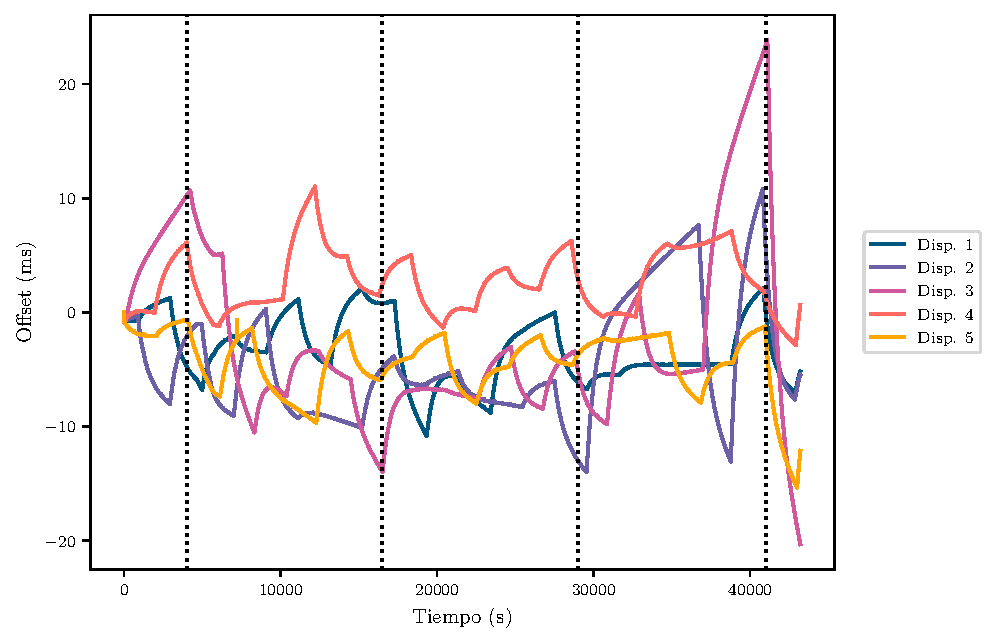
\includegraphics[scale=0.65]{../Python/plots/parallel/offset_plot}
    \caption{Offset acumulado muestra paralela}
    \label{fig:off_acu_paralelo}
\end{figure}

Esta ``sincronización'' entre dispositivos parece deberse a algún tipo de actualización del reloj interno del dispositivo mediante algún demonio del sistema operativo. El principal demonio que se encarga de esta tarea es el servicio NTP, el cual fue desactivado para realizar estas pruebas. 

Consultando otro diagrama de cajas con el incremento de la desviación en cada instante (Fig. \ref{fig:box_paralelo}) se observa como todos los dispositivos están más a la par que en la muestra secuencial (Fig. \ref{fig:box_secuencial}). Aún así, siguen teniendo ciertas diferencias, con lo que se puede concluir que también son estadísticamente diferenciables.

\begin{figure}
    \centering
    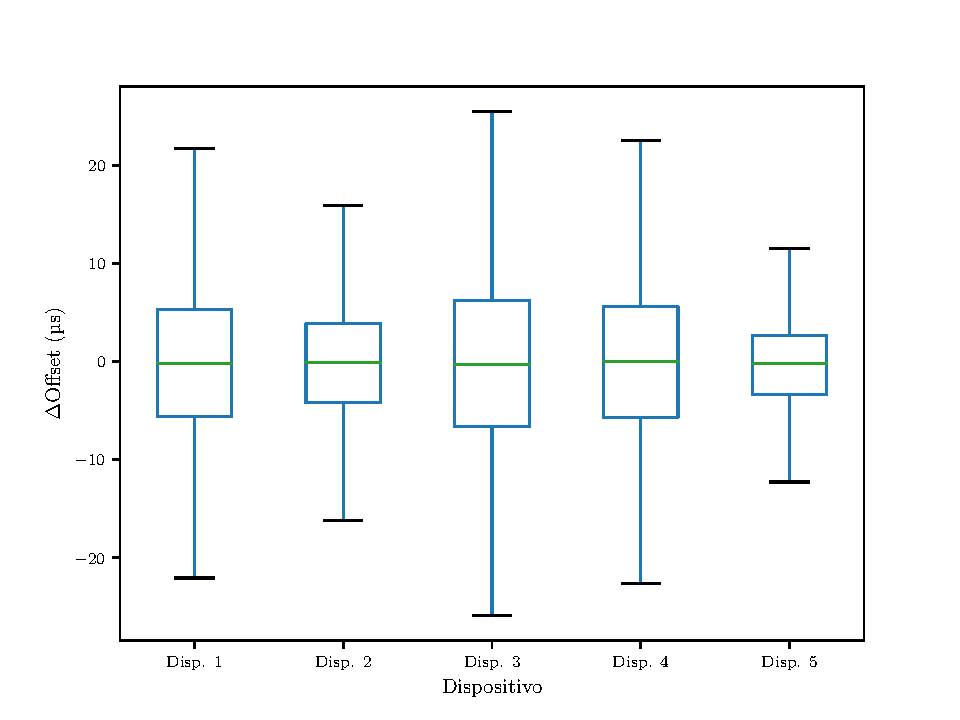
\includegraphics[scale=0.7]{../Python/plots/parallel/boxplot_no_out}
    \caption{Diagrama de cajas muestra paralela}
    \label{fig:box_paralelo}
\end{figure}

\section{Elección de la muestra de datos}

Analizando los incrementos de la desviación en ambas muestras se puede ver que la muestra paralela tiene valores más parecidos a los esperados. Estos valores de incremento de la desviación son más pequeños y más parecidos entre todos los dispositivos, es por ello que se entrenarán los algoritmos con los datos de la muestra paralela.

Estos datos se obtendrán mediante una ventana deslizante de \SI{1}{} minuto sobre el incremento de la desviación del reloj del dispositivo. Se obtendrán las siguientes variables estadísticas:
\begin{multicols}{2}
    \begin{itemize}
        \item Suma
        \item Media
        \item Mediana
        \item Moda
        \item Desviación típica
        \item Rango intercuartílico
        \item Curtosis
        \item Coeficiente de asimetría (skewness)
        \item Máximo
        \item Mínimo
    \end{itemize}
\end{multicols}

Generando estos datos estadísticos de la muestra paralela mediante la ventana deslizante, se obtienen los resultados que se pueden ver en la Tabla \ref{tab:stats_par}. Estos datos estadísticos serán los que posteriormente se usarán para entrenar un modelo de Machine Learning.

\begin{table}
    \centering
    \resizebox{0.85\textwidth}{!}{
        \begin{tabular}{cccccccccccc}
            \toprule
             & Sum & Mean & Median & Mode & Std & IQR & Kurtosis & Skew & Max & Min & Device \\
            \midrule
            1 & 21773.0 & 362.8833333333333 & -306.5 & -17885.0 & 8212.584818005707 & 12095.5 & 0.0567239505757037 & 0.4351150677774124 & 20799.0 & -17885.0 & Disp. 1 \\
            2 & 4059.0 & 67.65 & 239.5 & -15862.0 & 5615.809629134339 & 3012.25 & 1.400480680742287 & -0.1242668154207108 & 14194.0 & -15862.0 & Disp. 2 \\
            3 & 1187.0 & 19.78333333333333 & 503.5 & -25009.0 & 7760.832728977938 & 8467.0 & 1.231550787741679 & -0.2621794660161829 & 20510.0 & -25009.0 & Disp. 3 \\
            4 & 74154.0 & 1235.9 & 2016.5 & -21616.0 & 8391.731753359314 & 9663.75 & 0.4104874852336051 & -0.4087239664161064 & 19992.0 & -21616.0 & Disp. 4 \\
            5 & -127078.0 & -2117.9666666666667 & -2385.0 & -11894.0 & 4354.015072678016 & 2737.0 & 1.9665757630194 & 0.6070065306393123 & 10383.0 & -11894.0 & Disp. 5 \\
            6 & 20147.0 & 335.78333333333336 & -306.5 & -17885.0 & 8244.497450208664 & 12095.5 & 0.0362682762350909 & 0.4263535051366743 & 20799.0 & -17885.0 & Disp. 1 \\
            \vdots & \vdots & \vdots & \vdots & \vdots & \vdots & \vdots & \vdots & \vdots & \vdots & \vdots & \vdots \\
            \bottomrule
        \end{tabular}
    }
    \caption{Datos estadísticos muestra paralela}
    \label{tab:stats_par}
\end{table}

\section{Reducción de la dimensionalidad}

En esta sección buscaremos valores estadísticos correlacionados entre sí. En caso de existir habrá que eliminarlos antes de entrenar los modelos, puesto que no aportan información y provocarán que el algoritmo tarde aún más tiempo en ser entrenado.

La correlación entre las variables estadísticas se puede ver en la Fig. \ref{fig:corr}. Se puede ver como suma, media y mediana son las variables más correlacionadas entre sí, por tanto serán eliminadas 2 de ellas.

\begin{figure}
    \centering
    \subfloat[Correlación entre las variables iniciales]{
        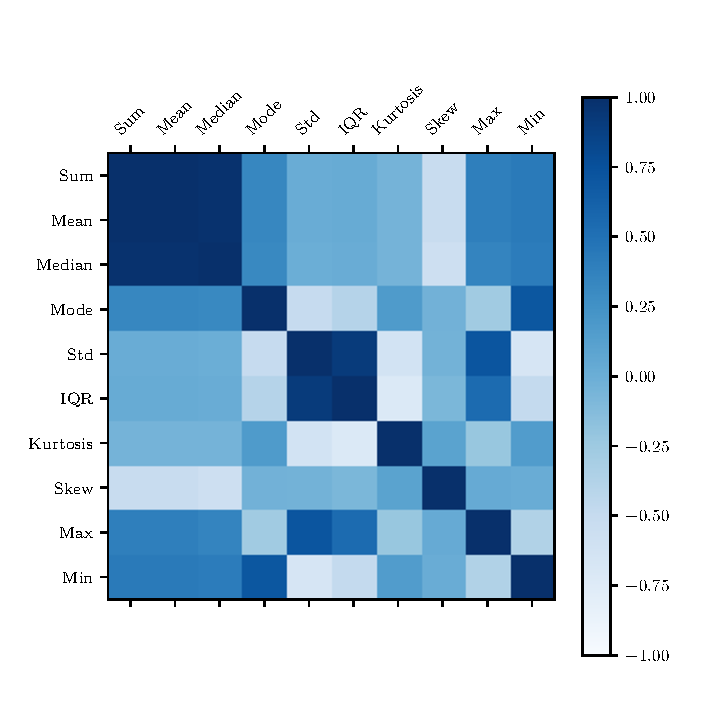
\includegraphics[scale=0.55]{../Python/plots/parallel/correlacion_stats.pdf}
    }
    \subfloat[Correlación entre las variables finales]{
        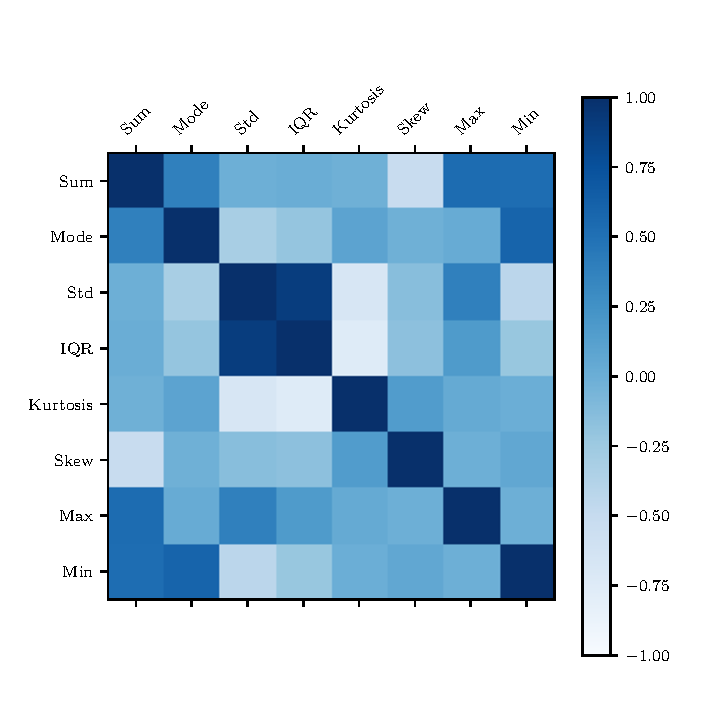
\includegraphics[scale=0.55]{../Python/plots/parallel/correlacion_stats_ftred.pdf}
    }
    \caption{Correlación entre las variables estadísticas}
    \label{fig:corr}
\end{figure} 

\section{Entrenamiento de los modelos}

En esta sección se analizarán los resultados que hemos obtenido de los modelos sobre los datos de la muestra paralela, como hemos concluido en la sección anterior.

Para realizar este entrenamiento se ha usado la librería \texttt{scikit-learn} sobre el lenguaje de programación Python. Esta librería tiene clases que implementan los algoritmos vistos anteriormente que serán los que se usarán (Sec. \ref{sec:algorithms}). Las clases que corresponden a cada modelo son las que se ven en la Tabla \ref{tab:equiv_models}.

\begin{table}
    \centering
    \begin{tabular}{cc}
        \toprule
        Algoritmo & Implementación \\
        \midrule
        Árboles de decisión & \texttt{DecisionTreeClassifier} \cite{scikittrees} \\
        Random Forest & \texttt{RandomForestClassifier} \cite{scikitforest} \\
        MLP & \texttt{MLPClassifier} \cite{scikitmlp} \\
        Naive Bayes & \texttt{GaussianNB} \cite{scikitnaivebayes} \\
        KNN & \texttt{KNeighborsClassifier} \cite{scikitknn} \\
        SVM & \texttt{LinearSVC} \cite{scikitsvm} \\
        \bottomrule
    \end{tabular}
    \caption{Equivalencia entre algoritmo e implementación}
    \label{tab:equiv_models}
\end{table}

\begin{figure}
    \centering
    \resizebox{0.5\textwidth}{!}{
    \begin{tikzpicture}
        \node[database,label=below:Datos,database radius=1cm,database segment height=0.5cm] (data) {};
        \node (aux) [right = of data] {};
        \node[database,label=below:Entrenamiento,database radius=0.75cm,database segment height=0.375cm] (train) [above right = 2cm of aux] {};
        \node[database,label=below:Test,database radius=0.75cm,database segment height=0.375cm] (test) [below right = 2cm of aux] {};
        \node[database,label=below:{$\underset{\text{Reducido}}{\text{Entrenamiento}}$},database radius=0.5cm,database segment height=0.25cm] (train2) [right = 3cm of train] {};
        \node (aux2) [right = of train2] {};
        \node[database,label=below:Entrenamiento,label=right:70\%,database radius=0.5cm,database segment height=0.25cm] (train3) [above right = of aux2] {};
        \node[database,label=below:Validación,label=right:30\%,database radius=0.5cm,database segment height=0.25cm] (test) [below right = of aux2] {};
        \draw[-] (1.2,0) -- (aux.center);
        \draw[-] (aux.center) |- (3.4, 2.4) node [above, pos=0.75] {70\%};
        \draw[-] (aux.center) |- (3.4, -2.45) node [below, pos=0.75] {30\%};
        \draw[-] (5.5, 2.4) -- (8, 2.4) node [midway, above] {35\%};
        \draw[-] (9.5, 2.4) -- (aux2.center);
        \draw[-] (aux2.center) |- (11.3, 4.1);
        \draw[-] (aux2.center) |- (11.3, 0.66);
    \end{tikzpicture}
    }
    \caption{Particiones de los datos}
    \label{fig:database}
\end{figure}

A la hora de entrenar modelos de machine learning lo primero que hay hacer es ajustar sus hiperparámetros. Los hiperparámetros de un modelo son parámetros del mismo que se pueden modificar para que este se adapte mejor a los datos con los que se está trabajando o para cambiar la forma en la aprende este modelo también para adaptarse a estos datos.

Para ajustar los hiperparámetros no se usa la completitud de los datos, se usa un modelo entrenamiento/validación/test. Los datos se han dividido en un conjunto de entrenamiento y otro de test, 70\% para entrenamiento y 30\% para test, lo habitual es tener en torno a una tercera parte de los datos para entrenamiento y el resto para test. Este proceso (Fig. \ref{fig:database}) se hace para comprobar la capacidad de generalización del modelo con datos que no haya visto nunca.

Para particionar los datos se tomarán muestras aleatorias, pero ordenadas para mantener la correlación temporal de los datos. Por ejemplo, ante el conjunto de datos $x_1, \dots, x_{20}$, una muestra aleatoria podría ser $x_{15}, x_8, x_3, x_{17}, x_5, x_{12}$ pero si estos datos presentan una correlación temporal, como es el caso de este trabajo, esta se pierde. Por tanto, los datos han de ser devueltos a su orden natural $x_3, x_5, x_8, x_{12}, x_{15}, x_{17}$. 

El conjunto de entrenamiento se usará únicamente con el modelo final y con los hiperparámetros ya ajustados, puesto que contiene una gran cantidad de datos. Para ajustar los hiperparámetros de cada modelo y comparar los modelos entre sí se usará un conjunto reducido de este, un 35\% de los datos de entrenamiento.

Este subconjunto de los datos de entrenamiento también será dividido en un conjunto de entrenamiento/test, aunque en este caso el conjunto test recibirá el nombre de  conjunto de validación. Se entrenarán los distintos algoritmos con estos conjuntos con el fin de ajustar los hiperparámetros y decidir el mejor entre todos ellos.

Para comprobar qué hiperparámetros son los que mejor se ajustan a los datos, se usará la función \texttt{GridSearchCV} \cite{scikitgrid} que permite que dados un algoritmo y un conjunto de valores para los hiperparámetros probar todas las combinaciones y obtener así un accuracy de cada uno, con lo que se pueden comparar y filtrar únicamente a los mejores. Esta función permite usar la validación cruzada. La validación cruzada 

A continuación se mostrará un ejemplo del proceso de ajustar los hiperparámetros de un modelo, en este caso se usará el algoritmo de Random Forest sobre los datos la muestra paralela. Los hiperparámetros que se han decido ajustar son:
\begin{itemize}
    \item \texttt{criterion}: función que mide la pureza de los nodos hijos.
    \item \texttt{max\_features}: número de características que se tienen en cuenta para realizar la división de un nodo.
    \item \texttt{n\_estimators}: número de árboles de decisión que participan en el algoritmo.
\end{itemize}

Para evitar que una rama entre en un bucle infinito debido a que no es capaz de dividir correctamente los nodos se ha fijado la profundidad máxima de cada rama (hiperpárametro \texttt{max\_depth}) a un valor de 1000. 

Hablando en primer lugar sobre los hiperparámetros \texttt{criterion} y \texttt{max\_features} (Fig. \ref{fig:comp_hiperparam1}) se puede ver que en promedio el mejor valor de \texttt{criterion} es \texttt{gini}. Este parámetro será fijado y, a continuación, se comprobarán todos los pares de valores que generan los hiperparámetros \texttt{max\_features} y \texttt{n\_estimators} (Fig. \ref{fig:comp_hiperparam2}).

\begin{figure}
    \centering
    \subfloat[]{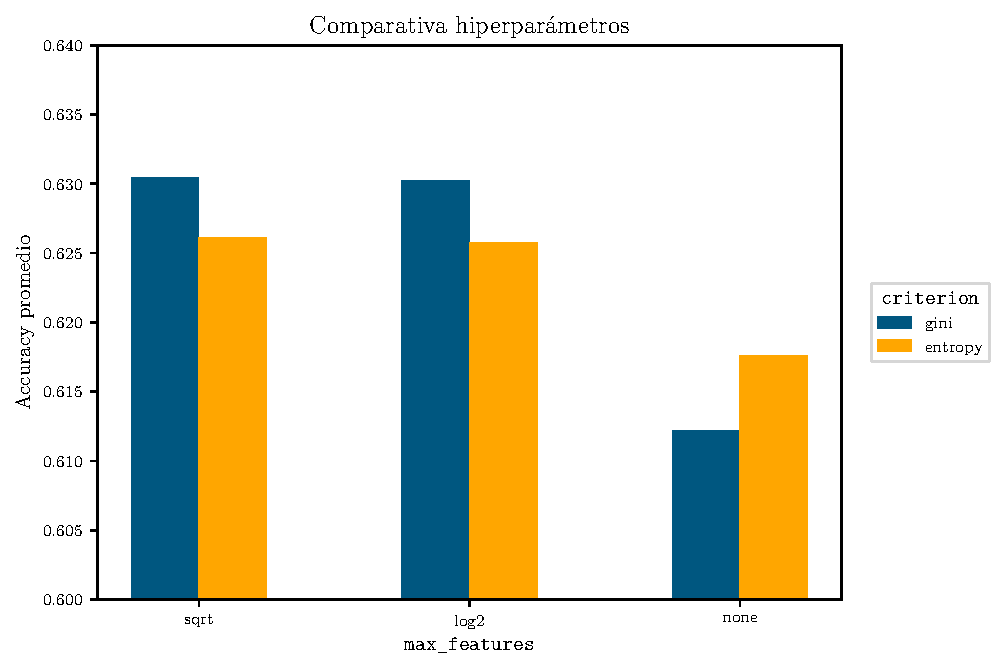
\includegraphics[width=0.45\textwidth]{../Python/plots/parallel/delta_random_forest_results}\label{fig:comp_hiperparam1}}
    \quad
    \subfloat[]{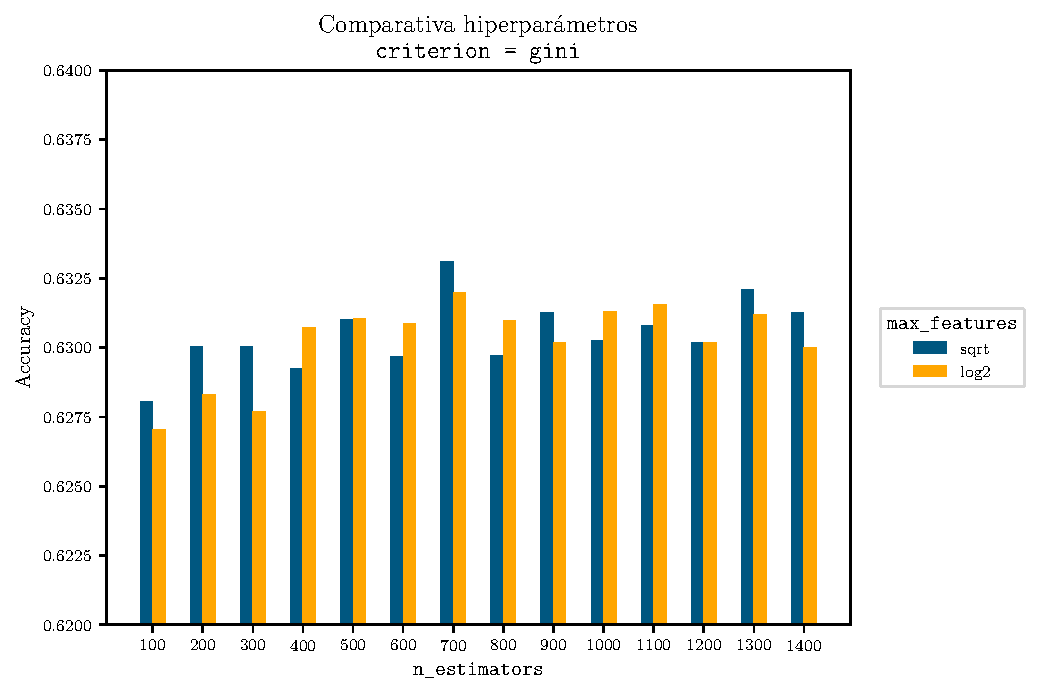
\includegraphics[width=0.45\textwidth]{../Python/plots/parallel/delta_random_forest_results2}\label{fig:comp_hiperparam2}}
    \caption{Comparativa hiperparámetros Random Forest}
    \label{fig:comp_hiperparam}
\end{figure}

Los mejores valores obtenidos son \texttt{criterion = gini}, \texttt{n\_estimators = 700} y \texttt{max\_features = sqrt}. Con estos hiperparámetros se entrenará un modelo sobre el conjunto de entrenamiento menor y después se realizará una predicción con el conjunto de validación.



% Análisis de los resultados
%!TEX root = TFG.tex

\chapter{Resultados} \label{chap:result}

Una vez entrenados todos los algoritmos con sus mejores hiperparámetros y con un valor de generalización obtenido de la predicción, tenemos los resultados que se pueden ver en la Fig. \ref{fig:comp_accur}.

\begin{figure}
    \centering
    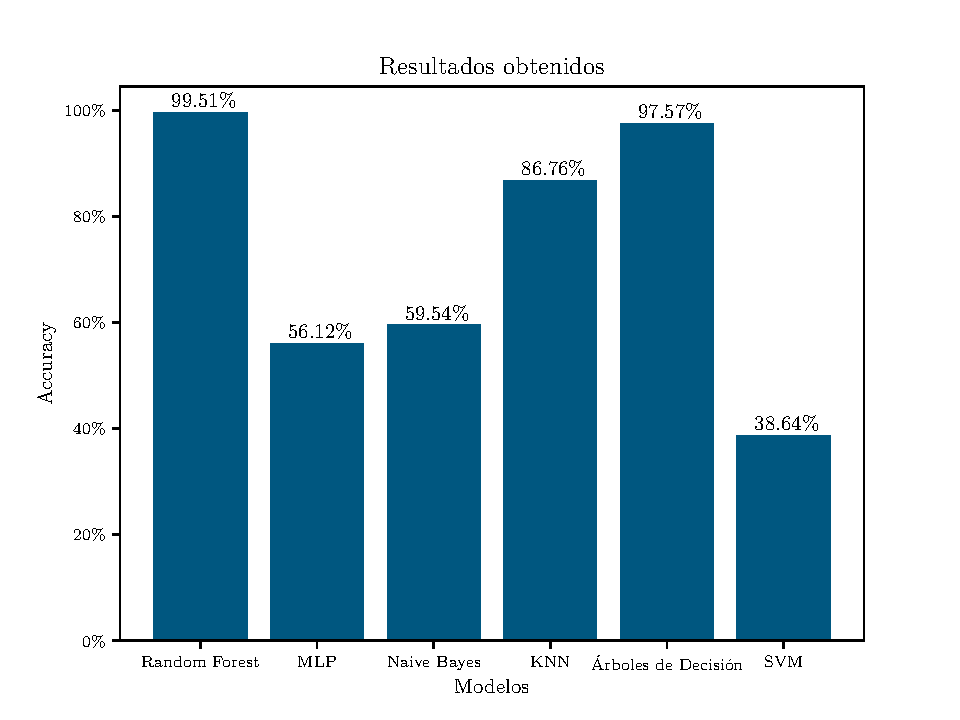
\includegraphics[width=0.4\textwidth]{../Python/plots/parallel/accur_results}
    \caption{Comparativa de resultados entre modelos}
    \label{fig:comp_accur}
\end{figure}

Como se puede ver en ambas muestras los modelos que presentan mejores resultados son los que se basan en árboles de decisión, que son el propio algoritmo de árboles de decisión y random forest. Otra forma de ver estos resultados es mediante las matrices de confusión que nos genera cada algoritmo.

\begin{figure}
    \centering
    \begin{tabular}{ccc}
        \subfloat{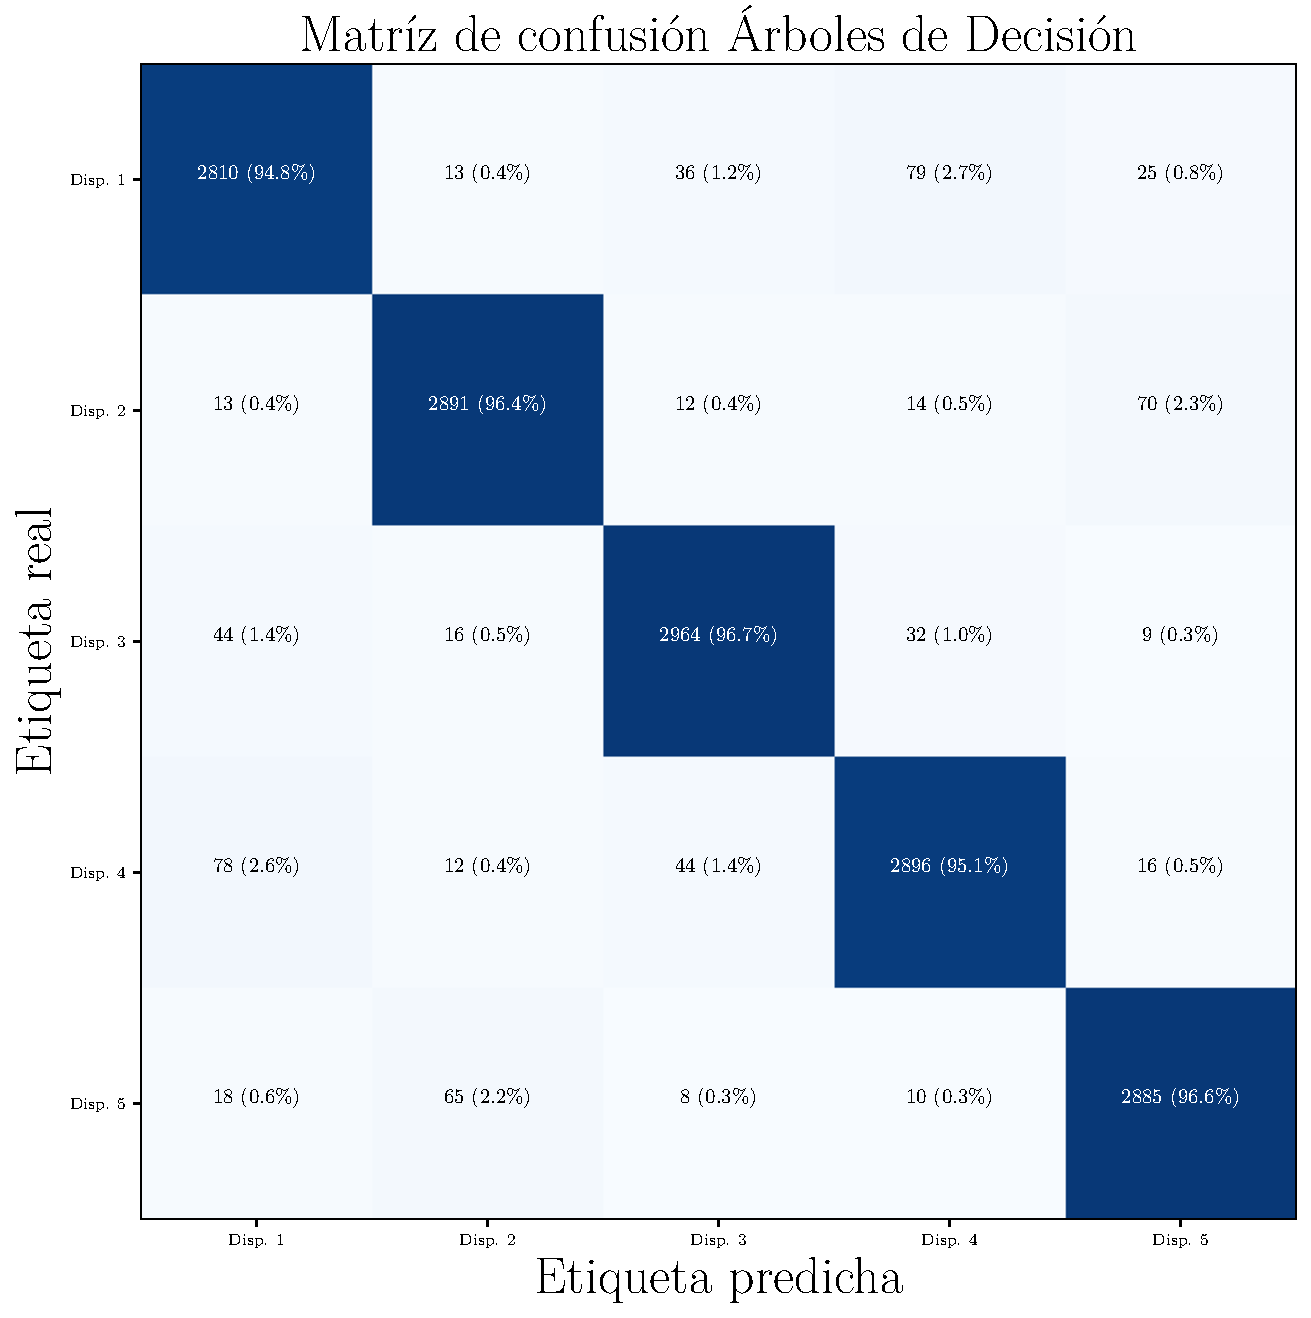
\includegraphics[width=0.4\textwidth]{../Python/plots/parallel/decision_tree_matrix}} & \subfloat{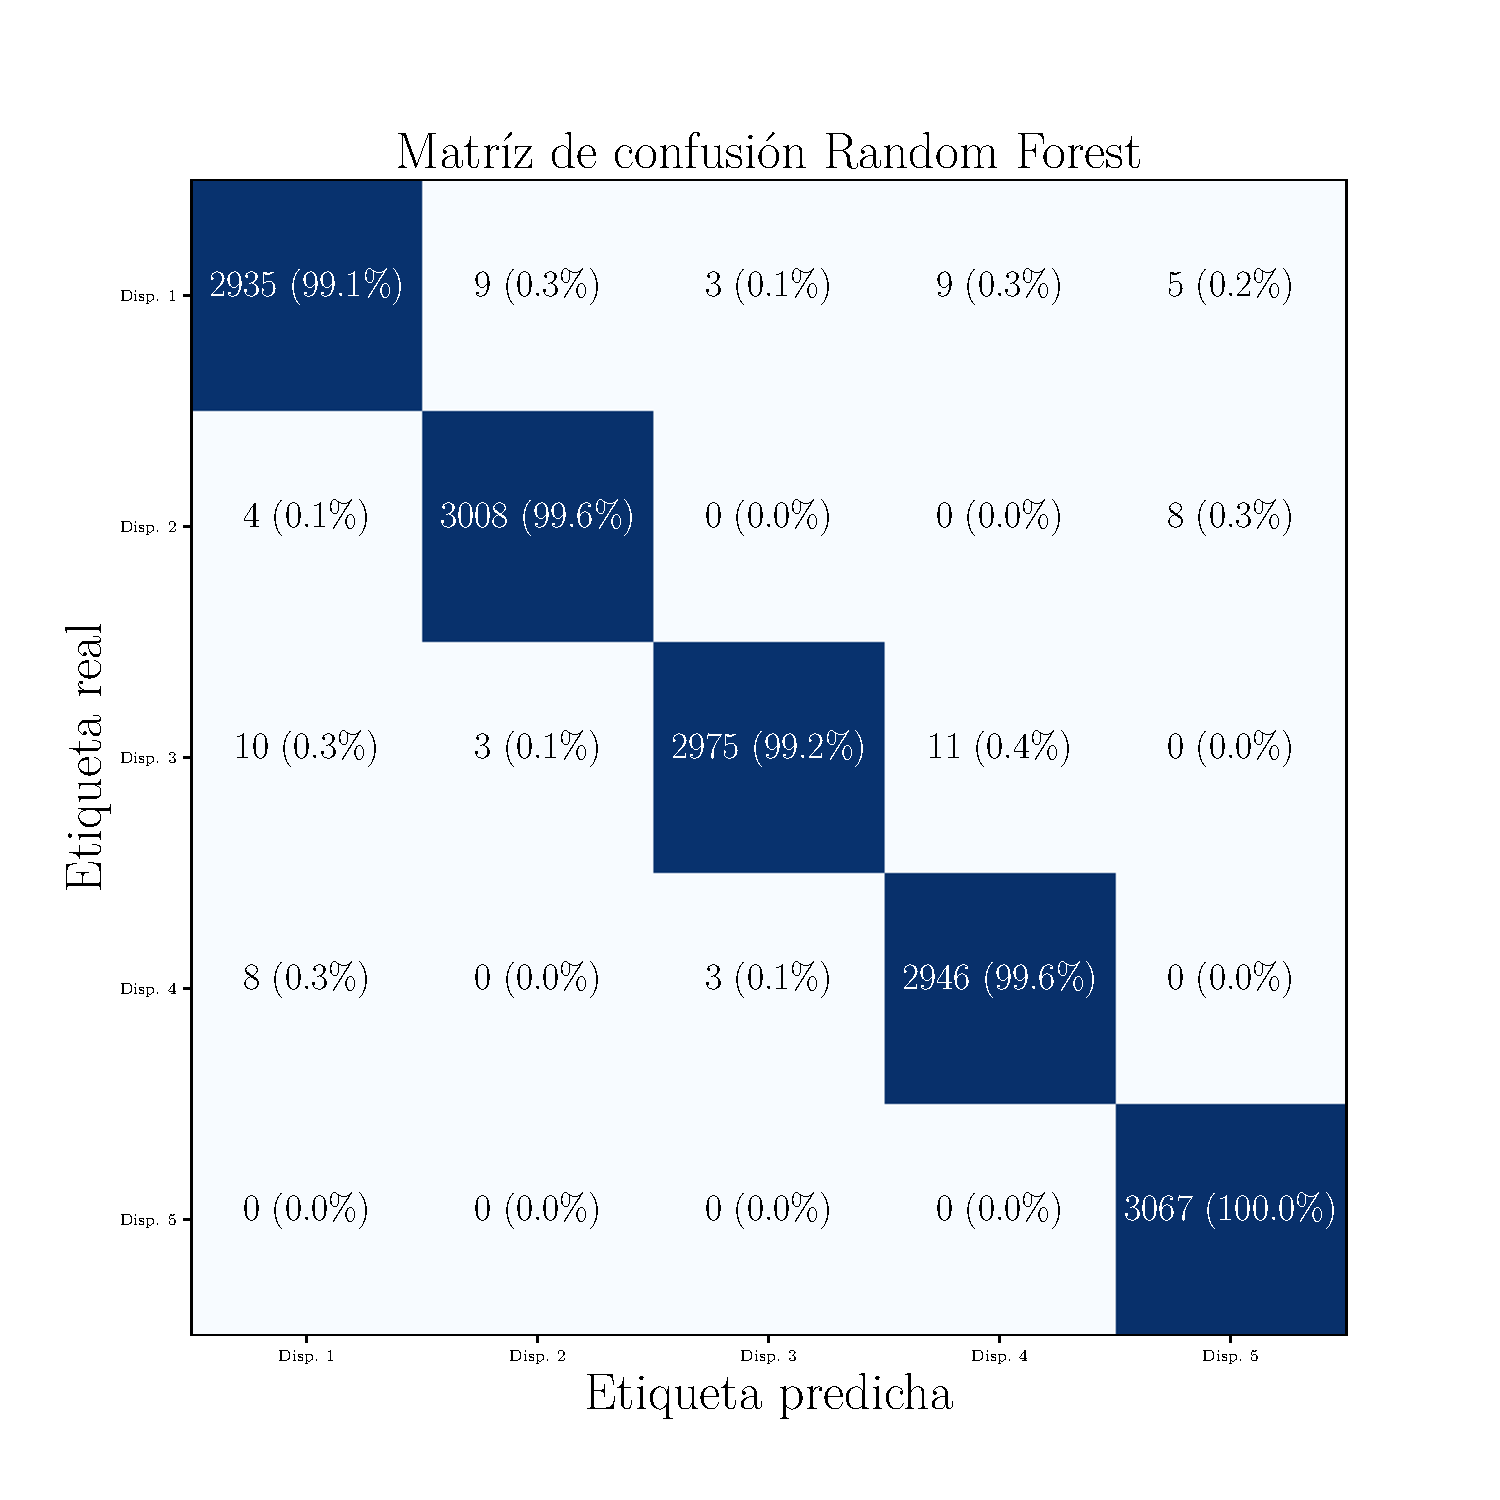
\includegraphics[width=0.4\textwidth]{../Python/plots/parallel/random_forest_matrix}} & \multirow{3}{*}[8em]{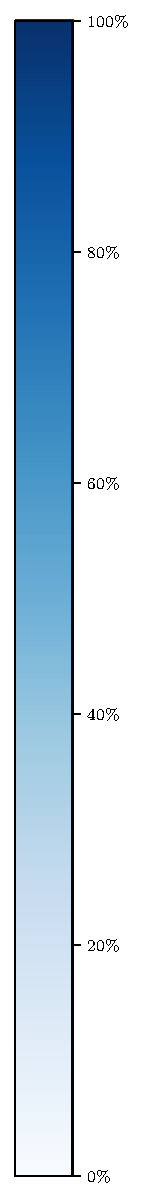
\includegraphics[scale=0.75]{../Python/plots/parallel/colorbar_matrices}} \\
        \subfloat{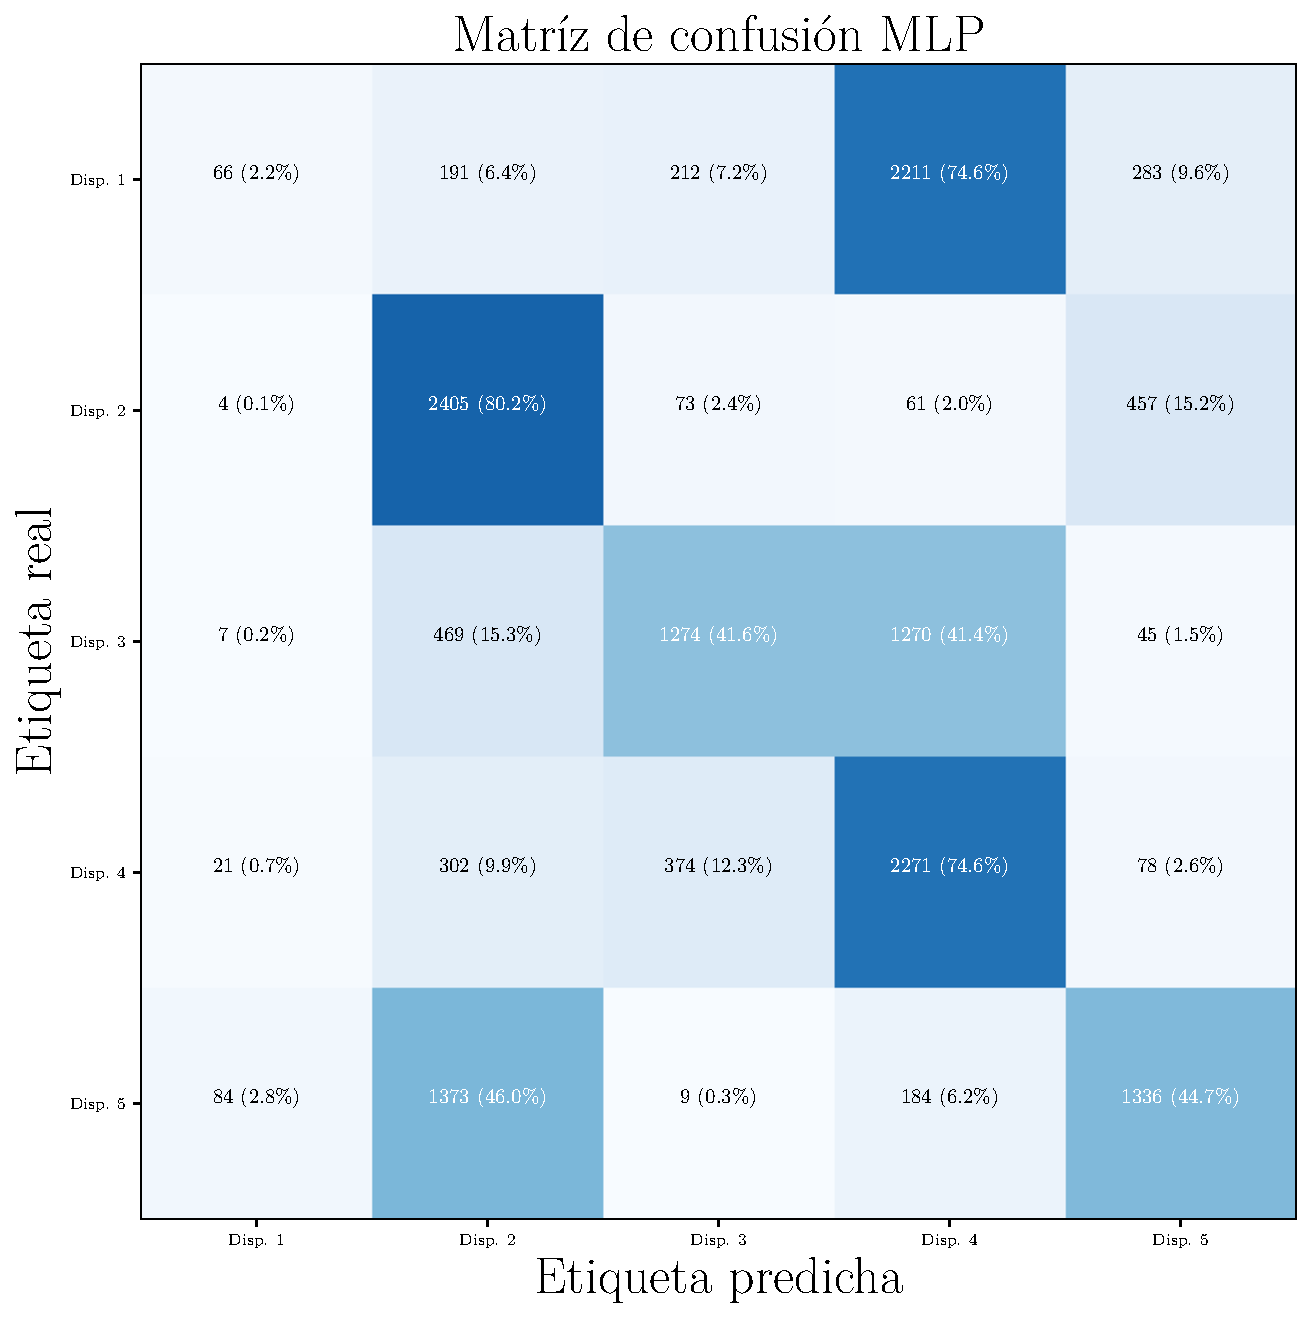
\includegraphics[width=0.4\textwidth]{../Python/plots/parallel/mlp_matrix}} & \subfloat{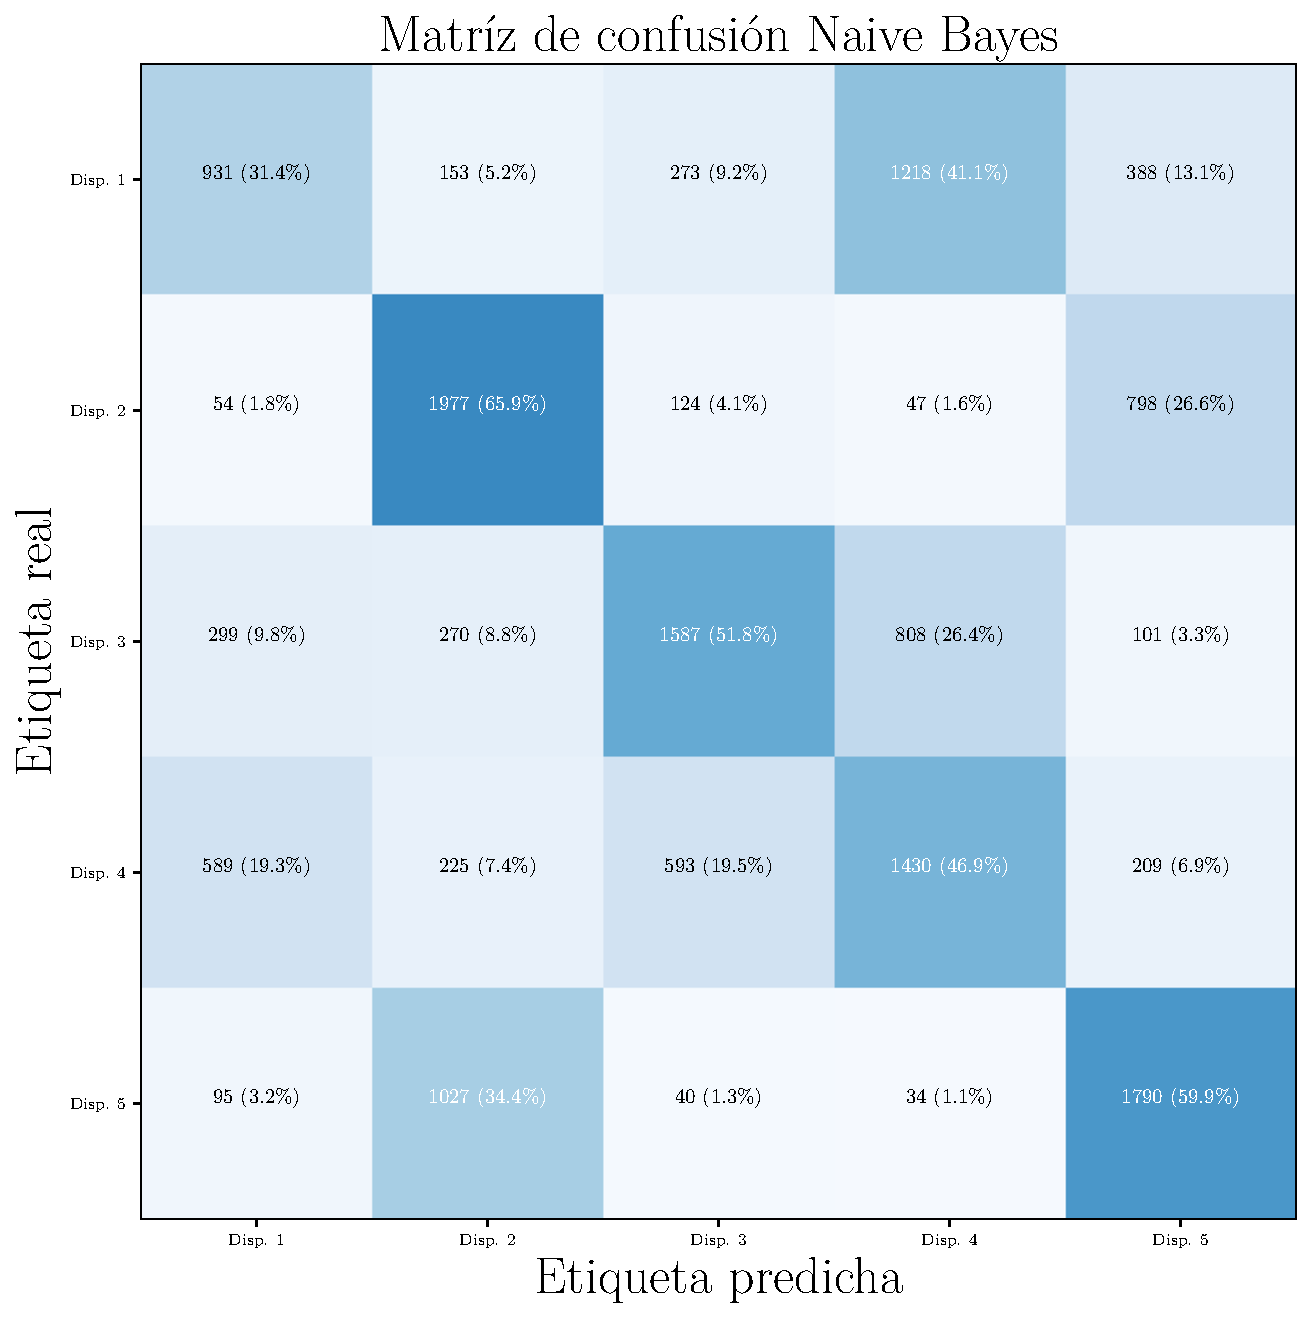
\includegraphics[width=0.4\textwidth]{../Python/plots/parallel/naive_bayes_matrix}} &  \\
        \subfloat{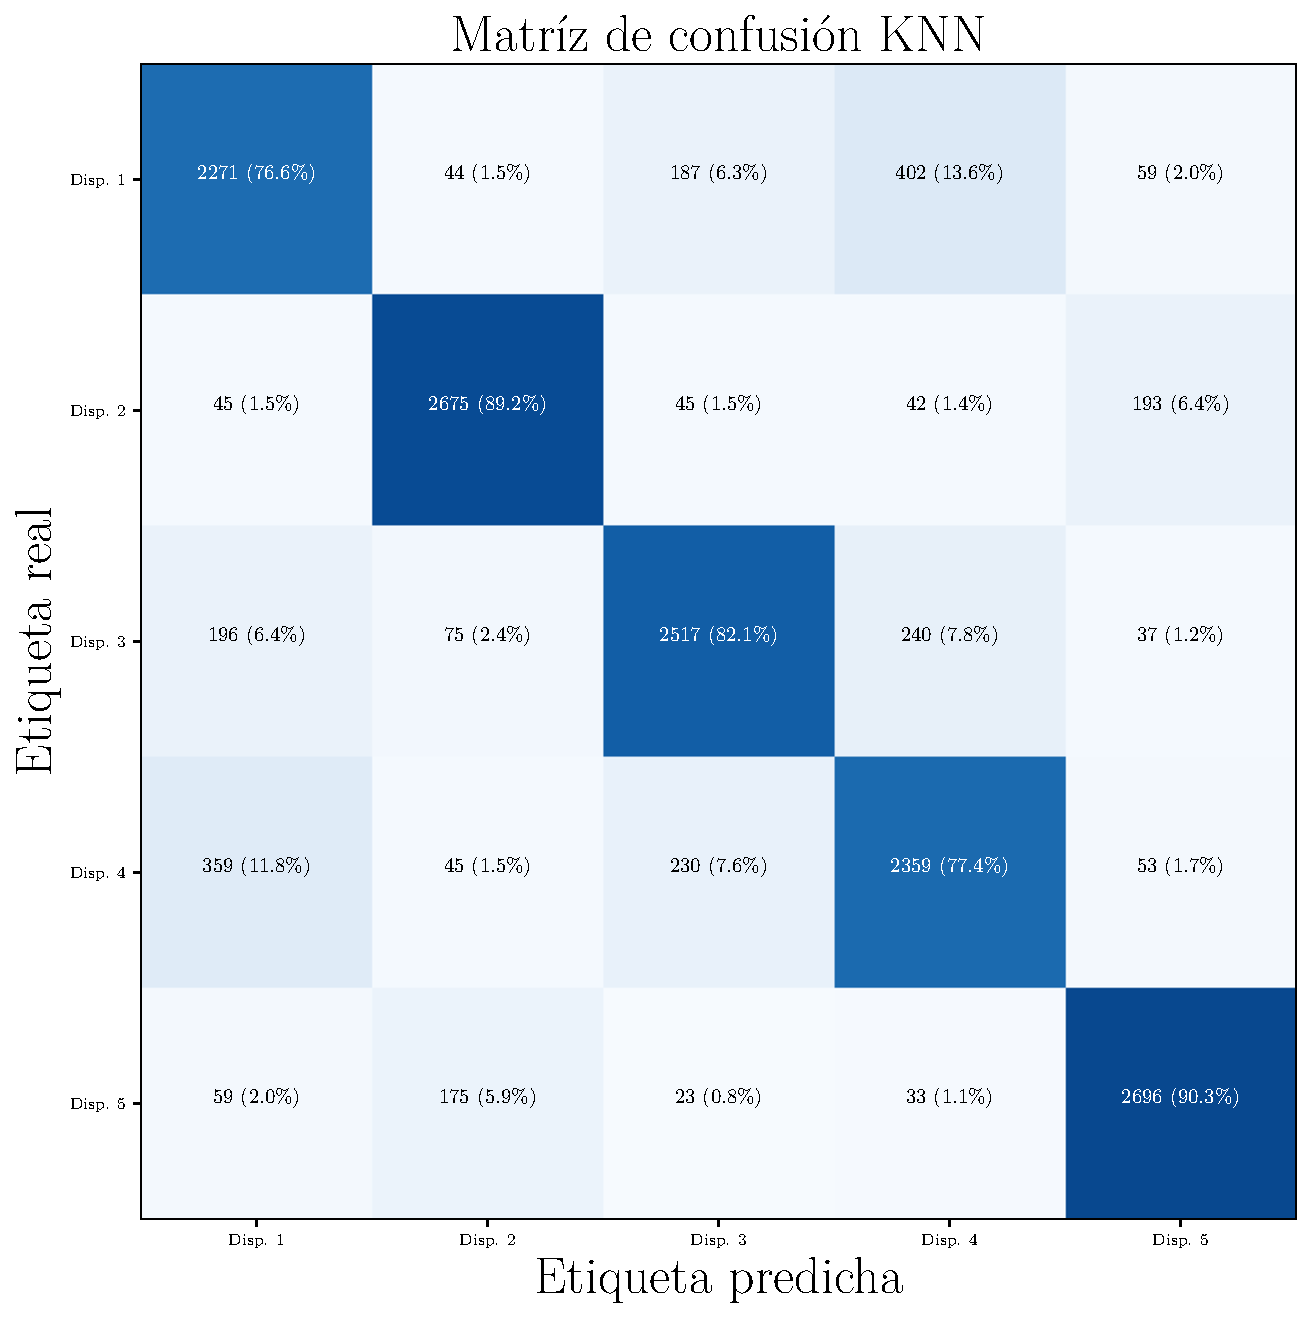
\includegraphics[width=0.4\textwidth]{../Python/plots/parallel/knn_matrix}} & \subfloat{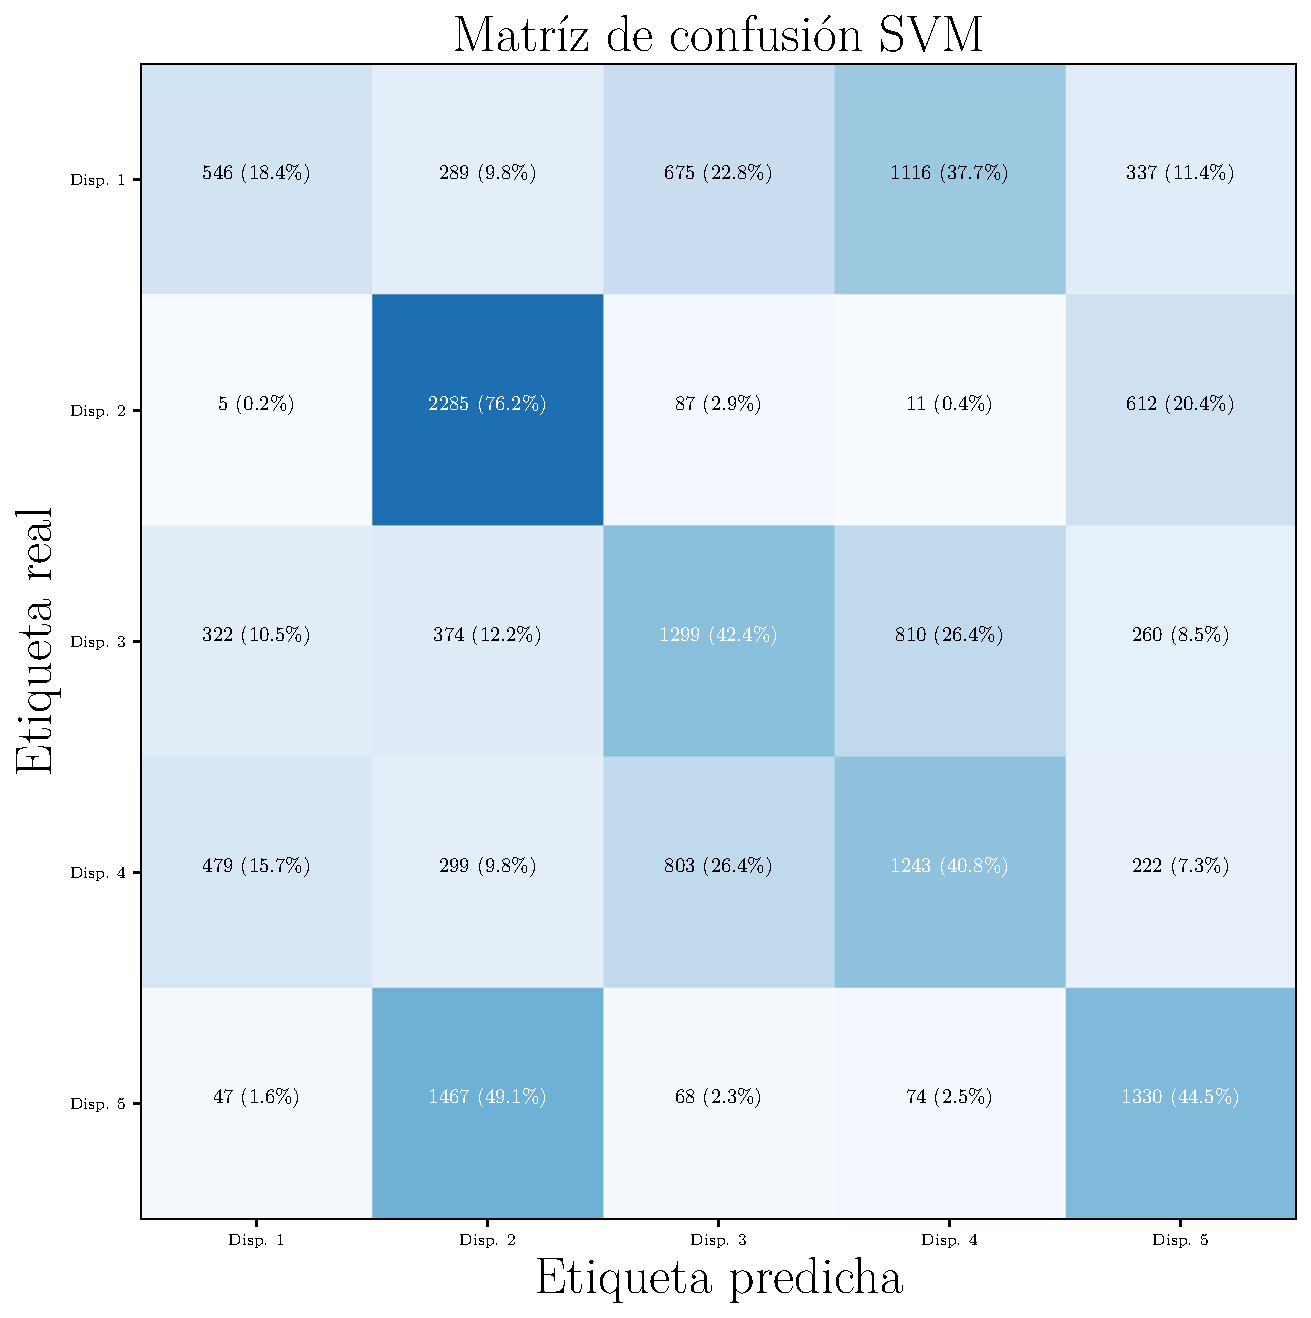
\includegraphics[width=0.4\textwidth]{../Python/plots/parallel/svm_linear_matrix}} & \\
    \end{tabular}
    \caption{Matrices de confusión con datos de la muestra paralela}
    \label{fig:confusion_matrices_parallel}
\end{figure}

Es fácil ver en la Fig. \ref{fig:confusion_matrices_parallel} que los modelos basados en árboles aciertan prácticamente en la totalidad de las ocasiones, en particular, el algoritmo de random forest es el que mejores resultados consigue ($\sim 99.5\%$). Por esta razón se entrenará un modelo de random forest con los hiperparámetros ajustados anteriormente con la totalidad de los datos de entrenamiento. Los resultados obtenidos se pueden ver en la matriz de confusión resultante (Fig. \ref{fig:final_matrix}). Con estos resultados se tiene un valor final de accuracy de 99.44\%.

\begin{figure}[H]
    \centering
    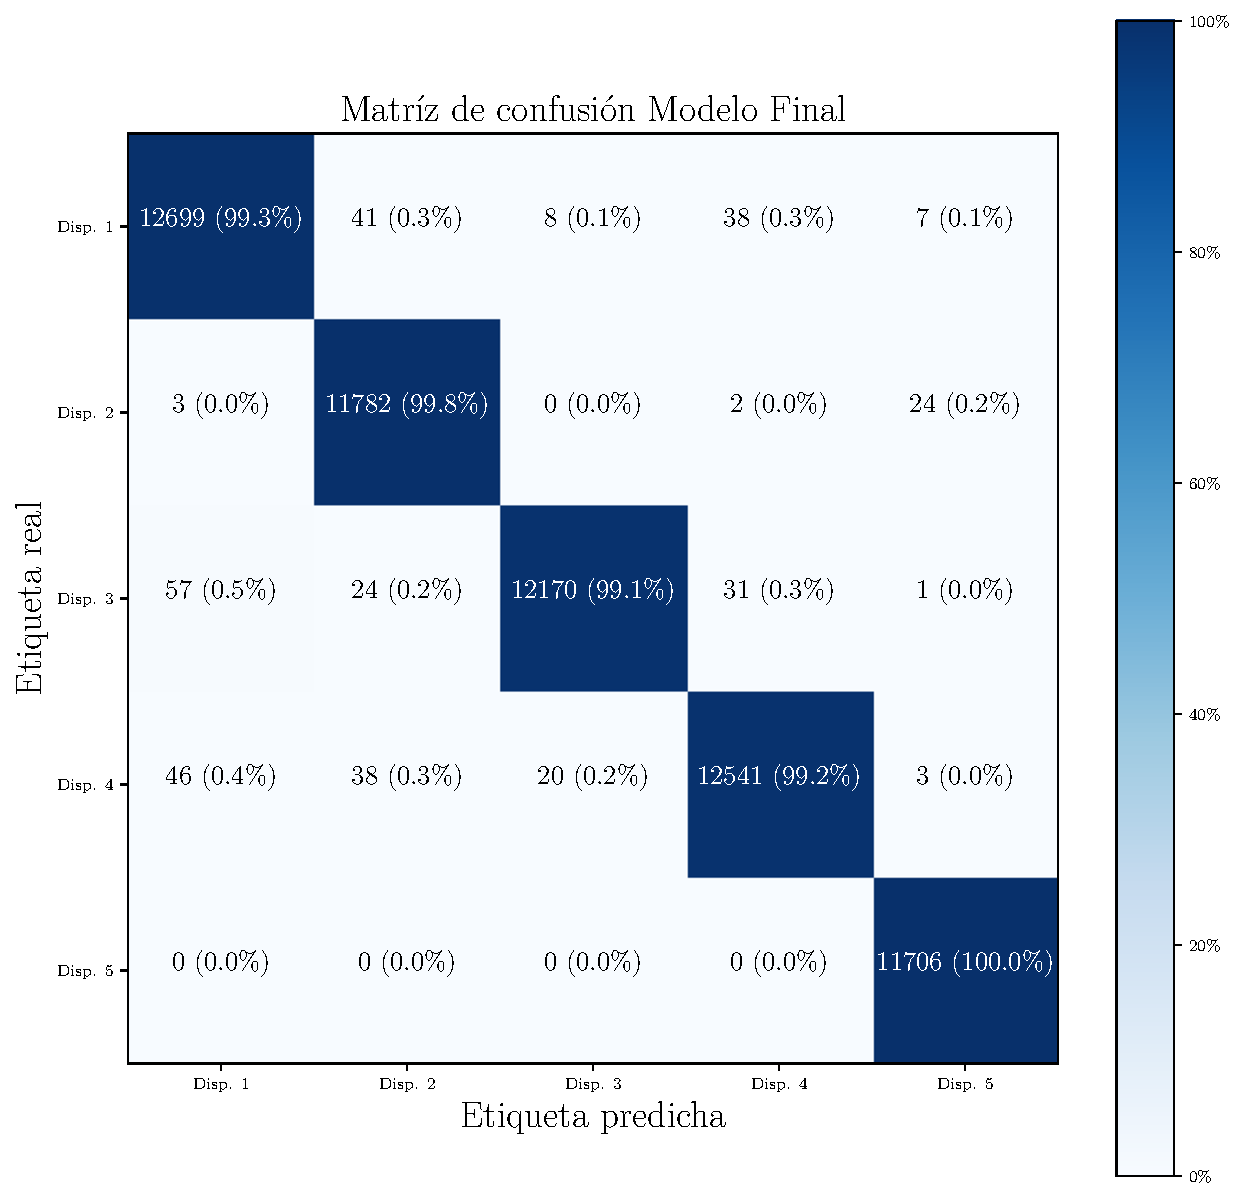
\includegraphics[scale=0.3]{../Python/plots/parallel/final_model_matrix}
    \caption{Matríz de confusión del modelo final}
    \label{fig:final_matrix}
\end{figure}


% Conclusiones y vias futuras
%!TEX root = TFG.tex

\chapter{Conclusiones y vías futuras} \label{chap:conclu}

En este proyecto hemos diseñado un modelo capaz de clasificar dispositivos con los que nos estamos comunicando en base a pequeñas diferencias en la fabricación de los componentes, que altera el tiempo que tardan en ejecutar una cierta tarea.

En la primera parte del proyecto hemos visto como para obtener la precisión en los tiempos que queríamos hemos tenido que usar el protocolo TCP y enviar las marcas de tiempo en el cuerpo del paquete. 

En este momento se vio que el interno es susceptible de ser alterado por procesos externos para que esté sincronizado en todo momento con el resto de los dispositivos (protocolo NTP), por este motivó este servicio tuvo que ser desactivado antes de realizar ninguna captura de paquetes, pues los diferencias entre tiempos no serían las propias del dispositivo.

Una vez desactivado el servicio, aún se obtenían datos que no eran correctos debido a que se estaba usando un reloj del sistema que podía ser modificado. Este reloj fue cambiado por un reloj que no fuera modificable (\texttt{steady\_clock}) y con eso los datos fueron más precisos.

Se realizaron capturas tanto en secuencial como en paralelo de la desviación de los relojes de los dispositivos, de las cuales se obtuvieron sus incrementos en cada momento. Con estos incrementos y una ventana deslizante de 1 minuto se obtienen variables estadísticas que servirán para entrenar los modelos.

Después de ver los resultados de los modelos con los conjuntos de entrenamiento/validación y analizando los posibles usos del sistema implementado se considera que es mejor quedarse con la muestra paralela. 

Por último entrenamos el modelo elegido, Random Forest, con los datos de la muestra paralela y los hiperparámetros que se consideraron mejores cuando se realizó el entrenamiento los conjuntos de entrenamiento/validación. De este modelo obtenemos unos resultados finales de 99.44\% en el valor de accuracy.

Como posibles vías futuras de este trabajo estaría el desarrollo de un modelo a tiempo real de este sistema. Para este cometido se debería tener una copia local de las huellas que generan ciertos dispositivos para poder compararlos con los que estamos recibiendo en ese momento y así comprobar si se trata de un atacante.

Para realizar este sistema a tiempo real también habría que crear mecanismos que permitan al sistema actualizarse con nuevos datos, y con ello generar nuevas huellas para los dispositivos. También habría que modificar los modelos de machine learning debido a que para que el sistema funcione a tiempo real, estos deberían actualizarse. 




% Apéndices, si hiciese falta
\appendix
%\include{apendice1.tex}

% Bibliografía
\selectlanguage{english}
\rhead{}
\lhead{}
\renewcommand\bibname{Bibliografía}
\printbibliography[heading = bibintoc]

\end{document}
